              %******************************************%
              %                                          %
              %     Modello di articolo scientifico      %
              %            di Luca Benvenuti             %
              %                                          %
              %         versione: 22 maggio 2013         %
              %                                          %
              %******************************************%
       

% I seguenti commenti speciali impostano:
% 1. utf8 come codifica di input,
% 2. PDFLaTeX come motore di composizione;
% 3. Articolo.tex come documento principale;
% 4. il controllo ortografico italiano per l'editor.

% !TEX encoding = UTF-8
% !TEX TS-program = pdflatex
% !TEX root = Articolo.tex
% !TEX spellcheck = it-IT

\documentclass[10pt,%                       % corpo del font principale
               a4paper,%                    % carta A4
             %  oneside,%                    % solo fronte
              twoside,%                    % fronte-retro
               ]{article}                  % classe report di KOMA-Script;
	   
			   
\usepackage{fancyhdr}
               
\usepackage[T1]{fontenc}                    % codifica dei font:
                                            % NOTA BENE! richiede una distribuzione *completa* di LaTeX,
                                          % per esempio TeXLive o MiKTeX *complete*

\usepackage[utf8]{inputenc}              % codifica di input; anche [latin1] va beneutf8
                                           % NOTA BENE! va accordata con le preferenze dell'editor


\usepackage{microtype}                     % microtipografia

\usepackage[italian,english]{babel}        % per scrivere in italiano e in inglese;
                                           % l'ultima lingua (l'italiano) risulta predefinita
                                           
\usepackage[binding=5mm]{layaureo}         % margini ottimizzati per l'A4; rilegatura di 5 mm


\usepackage{lmodern}  					   %new gerahrd
\usepackage{cleveref}  					   %new gerahrd
\usepackage{emptypage}     
\usepackage{indentfirst}                    % rientra il primo capoverso di ogni sezione

\usepackage{booktabs}                       % tabelle
\usepackage{tabularx}                       % tabelle di larghezza prefissata
\usepackage{graphicx}                       % immagini

\usepackage{subfig}                         % sottofigure, sottotabelle
\usepackage{caption}                        % didascalie

\usepackage{listings}                       % codici

\usepackage[font=small]{quoting}            % citazioni

\usepackage{amsmath,amssymb,amsthm}        % matematica
\usepackage{amsxtra,amstext,amsfonts}
\usepackage{amscd}						   %chimica

\usepackage[english]{varioref}              % riferimenti completi della pagina

\usepackage{mparhack,fixltx2e,relsize}      % finezze tipografiche
\usepackage[babel]{csquotes}
      
\usepackage[style=numeric-comp,hyperref,backref,backend=bibtex]{biblatex}
\bibliography{Bibliografia}                 % database di biblatex 
                                          
\usepackage{chngpage,calc}                 % centra il frontespizio
\usepackage[dvipsnames]{xcolor}             % colori
\usepackage{color}

\usepackage{lipsum}                        % testo fittizio

\usepackage{eurosym}                       % simbolo dell'euro

\usepackage[pdfa]{hyperref}                      % collegamenti ipertestuali

\usepackage{bookmark}                      % segnalibri
\usepackage[figuresright]{rotating}

\usepackage{array}

\usepackage{enumitem}

\usepackage{colortbl}

\usepackage{floatflt}
\usepackage{titlesec}

\usepackage{eurosym}  %indovina

\setcounter{tocdepth}{5} %to make it appears in TOC
\setcounter{secnumdepth}{5} %to make it numbered


\usepackage{acronym}
\usepackage{rotating}

%*********************************************************************************
% impostazioni-articolo.tex
% di Lorenzo Pantieri (2012)
% file che contiene le impostazioni dell'articolo
%*********************************************************************************


%*********************************************************************************
% Comandi personali
%*******************************************************
%\newcommand{\myName}{Lorenzo Pantieri}                            % autore
\newcommand{\myTitle}{Characterization of Particle Based Simulation Parameters
by means of Artificial Neural Networks}  % titolo
\date{}                                                           % nessuna data

%\title{\myTitle}
%\author{\myName}



%*********************************************************************************
% Impostazioni di amsmath, amssymb, amsthm
%*********************************************************************************

% comandi per gli insiemi numerici (serve il pacchetto amssymb)
\newcommand{\numberset}{\mathbb} 
\newcommand{\N}{\numberset{N}} 
\newcommand{\R}{\numberset{R}} 

% un ambiente per i sistemi
\newenvironment{sistema}%
  {\left\lbrace\begin{array}{@{}l@{}}}%
  {\end{array}\right.}

% definizioni (serve il pacchetto amsthm)
\theoremstyle{definition} 
\newtheorem{definizione}{Definizione}

% teoremi, leggi e decreti (serve il pacchetto amsthm)
\theoremstyle{plain} 
\newtheorem{teorema}{Teorema}
\newtheorem{legge}{Legge}
\newtheorem{decreto}[legge]{Decreto}
\newtheorem{murphy}{Murphy}[section]



%*********************************************************************************
% Impostazioni di biblatex
%*********************************************************************************
\defbibheading{bibliography}{%
\phantomsection
\addcontentsline{toc}{section}{\refname}
\section*{\bibname\markboth{\MakeUppercase{\refname}}{\MakeUppercase{\refname}}}}



%*********************************************************************************
% Impostazioni di listings
%*********************************************************************************
\lstset{language=[LaTeX]Tex,%C++,
    keywordstyle=\color{RoyalBlue},%\bfseries,
    basicstyle=\small\ttfamily,
    %identifierstyle=\color{NavyBlue},
    commentstyle=\color{Green}\ttfamily,
    stringstyle=\rmfamily,
    numbers=none,%left,%
    numberstyle=\scriptsize,%\tiny
    stepnumber=5,
    numbersep=8pt,
    showstringspaces=false,
    breaklines=true,
    frameround=ftff,
    frame=single
} 



%*********************************************************************************
% Impostazioni di hyperref
%*********************************************************************************
% \hypersetup{%
%     hyperfootnotes=false,pdfpagelabels,
%     %draft,	% = elimina tutti i link (utile per stampe in bianco e nero)
%     colorlinks=true, linktocpage=true, pdfstartpage=1, pdfstartview=FitV,%
%     % decommenta la riga seguente per avere link in nero (per esempio per la stampa in bianco e nero)
%     %colorlinks=false, linktocpage=false, pdfborder={0 0 0}, pdfstartpage=1, pdfstartview=FitV,% 
%     breaklinks=true, pdfpagemode=UseNone, pageanchor=true, pdfpagemode=UseOutlines,%
%     plainpages=false, bookmarksnumbered, bookmarksopen=true, bookmarksopenlevel=1,%
%     hypertexnames=true, pdfhighlight=/O,%nesting=true,%frenchlinks,%
%     urlcolor=webbrown, linkcolor=RoyalBlue, citecolor=webgreen, %pagecolor=RoyalBlue,%
%     %urlcolor=Black, linkcolor=Black, citecolor=Black, %pagecolor=Black,%
%     pdftitle={\myTitle},%
%     pdfauthor={\textcopyright\ \myName},%
%     pdfsubject={},%
%     pdfkeywords={},%
%     pdfcreator={pdfLaTeX},%
%     pdfproducer={LaTeX with hyperref and ClassicThesis}%
% }



%*********************************************************************************
% Impostazioni di graphicx
%*********************************************************************************
%\graphicspath{{Immagini/}} % cartella dove sono riposte le immagini



%*********************************************************************************
% Impostazioni di xcolor
%*********************************************************************************
\definecolor{webgreen}{rgb}{0,.5,0}
\definecolor{webbrown}{rgb}{.6,0,0}



%*********************************************************************************
% Impostazioni di caption
%*********************************************************************************
\captionsetup{tableposition=top,figureposition=bottom,font=small,format=hang,labelfont=bf}



%*********************************************************************************
% Altro
%*********************************************************************************

% [...] ;-)
\newcommand{\omissis}{[\dots\negthinspace]}

% eccezioni all'algoritmo di sillabazione
\hyphenation{Fortran ma-cro-istru-zio-ne nitro-idrossil-amminico}

\pagenumbering{gobble} %to switch off page numbering.               % file con le impostazioni personali



\begin{document}
\pagestyle{headings} 
%******************************************************************
% Materiale iniziale
%******************************************************************
% !TEX encoding = UTF-8
% !TEX TS-program = pdflatex
% !TEX root = ../Articolo.tex
% !TEX spellcheck = it-IT

%*******************************************************
% Frontespizio
%*******************************************************
\begin{titlepage}
\pdfbookmark{Frontespizio}{Frontespizio}
\changetext{}{}{}{((\paperwidth - \textwidth) / 2) - \oddsidemargin - \hoffset - 1in}{}

\begin{center}


% Upper part of the page

\includegraphics[width=0.3\textwidth]{045PFM_Logo_Original}\\[1cm]    

\textsc{\LARGE \myDepartment}\\[1.5cm]


% This document uses the following counting scheme
%    I   - Year for Q1 of the year Year
%    II  - Year ...
%    III - Year
%    IV  - Year
\textsc{\Large \myTitle ~ - \RM{8}  - 2015}\\[0.5cm]


% Title
\HRule \\[0.4cm]
{ \huge \bfseries \myPhd}\\[0.4cm]

\HRule \\[1.5cm]

% Author and supervisor

\begin{minipage}{0.8\textwidth}
\begin{center} \large

\emph{Author:}\\[0.4cm]

%irstname \textsc{Lastname}
\myName \\
\texttt{\myemail}\\[1.5cm]

\emph{Supervisors:} \\[0.4cm]

\myProf \\[0.2cm]
\myOtherProf \\ [0.2cm]
%\end{flushright}

\end{center}

\end{minipage}

\vfill

% Print the current date at the bottom of the page
{\large \myTime}

\end{center}

\end{titlepage}

% !TEX encoding = UTF-8
% !TEX TS-program = pdflatex
% !TEX root = ../Articolo.tex
% !TEX spellcheck = it-IT

%*******************************************************
% Indici
%*******************************************************
\pdfbookmark{\contentsname}{tableofcontents}
\setcounter{tocdepth}{2}
\tableofcontents
\markboth{\contentsname}{\contentsname} 

%*******************************************************
% Elenco delle figure
%*******************************************************    
\phantomsection
\pdfbookmark{\listfigurename}{lof}
\listoffigures

%*******************************************************
% Elenco delle tabelle
%*******************************************************
\phantomsection
\pdfbookmark{\listtablename}{lot}
\listoftables
       
	   
\newpage
%
%% !TEX encoding = UTF-8
% !TEX TS-program = pdflatex
% !TEX root = ../Articolo.tex
% !TEX spellcheck = it-IT

%*******************************************************
% Sommario+Abstract
%*******************************************************
\phantomsection
\pdfbookmark{Sommario}{Sommario}
\section*{Sommario}

\lipsum[1]

\selectlanguage{english}
\pdfbookmark{Abstract}{Abstract}
\section*{Abstract}

\lipsum[2]

\selectlanguage{italian}


%******************************************************************
% Materiale principale
%******************************************************************

%% !TEX encoding = UTF-8
% !TEX TS-program = pdflatex
% !TEX root = ../Articolo.tex
% !TEX spellcheck = it-IT

%************************************************
\section{Scope of work}
\label{sec:scopeofwork}
%************************************************

The purpose of this PhD thesis is to utilize, develop and set up a handful of characterization devices.
These should be user friendly, as mechanized as possible (to avoid operator bias) and easy to set up, of course with the proper manuals that should also be written.\\
After the data collection physical key parameters of particle flows will be identified; 
this physical information should allow the calibration of series of trustworthy numerical parameters for \ac{dem} (\ac{liggghts}) and FEM (CFDEMcoupling) reliable simulations.
The knowledge gained so far should be applied to industrial processes.\\

%% !TEX encoding = UTF-8
% !TEX TS-program = pdflatex
% !TEX root = ../Articolo.tex
% !TEX spellcheck = it-IT

%************************************************
\section{Stages}
\label{section:stages}
%************************************************

The work stages defined until now are the following:

\begin{enumerate}
\item{\textbf{References collection}, \textit{and literature study};}
\item{\textbf{DEM Characterization Workflow Coarse Particles}, \textit{based on existing experiments};}
\item{\textbf{Set up of a Jenike shear cell}, \textit{through a training trip to the University of Braunschweig};}
\item{\textbf{DEM Characterization Workflow Powder}, \textit{temptative approach with the hollow sphere experiment};}
\item{\textbf{CFD Characterization Workflow Coarse Particles}, \textit{pressure drop in packed bed; lateral jet experiment};}
\item{\textbf{CFD Characterization Workflow Powder}, \textit{maybe thanks to the fluidized bed experiment};}
\item{\textbf{Sinter plant simulation}, \textit{the first application};}
\item{\textbf{Blast furnace simulation}, \textit{the second application};}
\item{\textbf{Conclusions writing};}
\end{enumerate}

%% !TEX encoding = UTF-8
% !TEX TS-program = pdflatex
% !TEX root = ../Articolo.tex
% !TEX spellcheck = it-IT

%************************************************
\section{References collection}
\label{section:referencescollection}
%************************************************

The first step of work has been the collection of some of the books and articles that concern the subject analyzed.
They can be found in the \hyperref[section:bibliography]{bibliography section (\ref{section:bibliography})}.\\

%% !TEX encoding = UTF-8
% !TEX TS-program = pdflatex
% !TEX root = ../Articolo.tex
% !TEX spellcheck = it-IT

%************************************************
\section{Conferences}
\label{sec:cfdconference}
%************************************************

For the rest of 2015 the conferences planned are as follow:
\begin{itemize}
\item{Particles 2015, Barcellona: participation confirmed;}
\item{EANN 2015, Rhodes, participation confirmed;}
\item{CFD 2015, Melbourne, paper sent for revision.}
\end{itemize}

%% !TEX encoding = UTF-8
% !TEX TS-program = pdflatex
% !TEX root = ../Articolo.tex
% !TEX spellcheck = it-IT

%************************************************
\section{Materials}
\label{section:materials}
%************************************************

With the agreement of the industrial partners, the range of the raw materials to be characterized has been extended until 50 mm of diameter.
Especially, we have also added lump ore.\\

%% !TEX encoding = UTF-8
% !TEX TS-program = pdflatex
% !TEX root = ../Tesi.tex
% !TEX spellcheck = it-IT

%************************************************
\chapter{DEM Parameters}
\label{cap:demparameters}
%************************************************

\lipsum[1]

\section{Literature Values}
\label{sec:literaturevalues}

\lipsum[1]

\section{Particle Distribution}
\label{sec:particledistribution}

\lipsum[1]

% \subsection{coke}
% \label{subsec:coke}
% 
% \lipsum[2]

% \section{Bulk Density}
% \label{sec:bulkdensity}


\lipsum[1]


\section{Angle of Repose (p-p) - Small Scale}
\label{sec:aor}


\lipsum[1]

\section{Angle of Repose (p-p) - Large Scale}
\label{sec:aorlargescale}


\lipsum[1]

\section{Angle of Repose Simulation}
\label{sec:aorsimulation}


\lipsum[1]

% \section{Maximum Static Angle (p-w)}
% \label{sec:msa}
% %************************************************
% 
% \lipsum[1]
% 
% \section{Maximum Static Angle Simulation}
% \label{sec:msasimulation}
% %************************************************
% 
% \lipsum[1]

\section{Schulze Ring Shear Cell tester (p-p)}
\label{sec:SRSCT}
%************************************************

\lipsum[1]

\section{Jenike Shear Cell tester}
\label{sec:jsct}
%************************************************

\lipsum[1]

% \subsection{p-p}
% \label{subsec:JSCTpp}
% 
% \lipsum[2]
% 
% % \subsubsection{Instructions}
% % \label{subsubsec:instructions}
% % 
% % \paragraph{Scope}
% % \label{paragraph:scope}
% 
% \subsection{p-w}
% \label{subsec:JSCTpw}

\lipsum[3]

\section{Shear Cell Simulation}
\label{sec:scsimulation}
%************************************************

\lipsum[1]


% \section{Coefficient of Restitution}
% \label{sec:COR}
% %************************************************
% 
% \lipsum[1]

% \subsection{p-p}
% \label{subsec:CORpp}
% 
% \lipsum[2]
% 
% \subsection{p-w}
% \label{subsec:CORpw}
% 
% \lipsum[3]

% \section{Coefficient of Restitution Simulation - Estimation Matlab}
% \label{sec:corsimulation}
% %************************************************

\lipsum[1]

% !TEX encoding = UTF-8
% !TEX TS-program = pdflatex
% !TEX root = ../Articolo.tex
% !TEX spellcheck = it-IT

%************************************************
\section{DEM Characterization Workflow Coarse Particles}
\label{section:Demcharacterizationworkflowcoarseparticles}
%************************************************

\subsection{Jenike's  Shear Cell tester}
\label{subsection:jenikeshearcell}

We have performed from 6 to 16 experiments per bulk material.\\

\subsubsection{SCT simulation}
\label{subsubsection:sctsimulation}

The script has been modified to run on 32 cores over $Mach$. As of now each shear cell experiment is simulated approx. 250 times with different combinations of parameters.
As can be seen in Fig. \ref{010dCylDpComparison}, a wall effect appears in the simulations, an the coefficient of internal friction decreases if the cell dimension grows. Since a bigger dimension means more particles and more computational demand, only a part of the simulations have been realized with a larger cell's diameter. The Neural Network, see section \ref{subsection:microparameters}, will account also for this $wall$ effect.\\
\begin{figure}[!h]
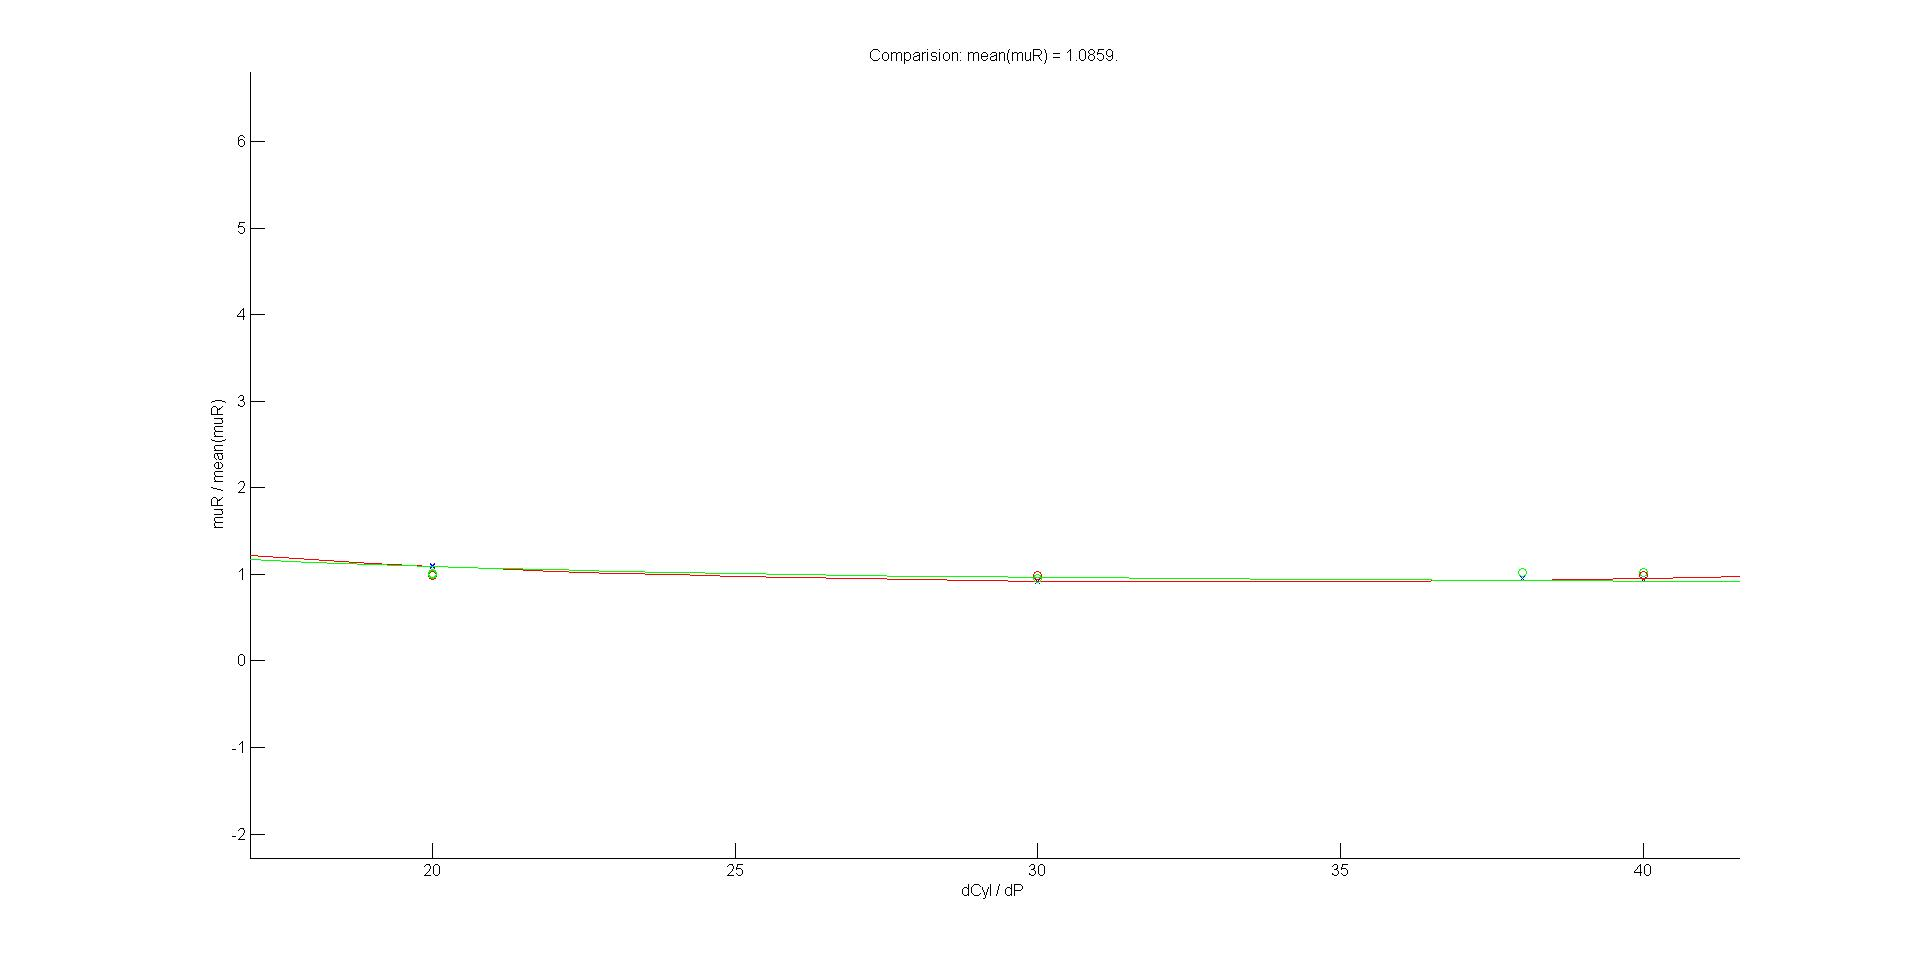
\includegraphics[width=.96\columnwidth]{010dCylDpComparison}
\caption{increased geometry effect}
\label{010dCylDpComparison}
\end{figure}

I received on the 10th of September this message from Mach: \textit{qsub: Maximum number of jobs for group k3b02 already in queue std.q}, with 35 scripts in queue (of them 14 are running, occupying 512 cores), when I tried to add a new script to the queue.
Now I have 18 scripts in queue (of them 7 are running, occupying 256 cores), but, since then, when I try to add a new script a receive the same error.
Since I am yet the only one in the department using Mach, I will contact the Administrator ASAP.\\

\subsection{Angle of Repose}
\label{subsection:aor}

For each bulk have been performed at least 2 experiments, of which the mean, median and variance values have been considered.\\

\subsubsection{AOR simulation}
\label{subsubsection:aorsimulation}

The script has been modified to run on 32 cores over $Mach$. As of now each material is simulated approx. 108 times with different combinations of parameters.\\

\subsection{Granulometric curves}
\label{subsection:granulometric curves}

I have completed sieving of all materials (except from 0 to 1.25 mm iron ore) and I have for them:
\begin{itemize}
\item{the granulometric curve;}
\item{the mean radius (R);}
\end{itemize}

\subsection{COR characterization}
\label{subsection:corcharacterization}

A new system based on frequency has been suggested. I will start working on it ASAP.

\subsection{Hollow spheres}
\label{subsection:hollowspheres}

This project will remain in stand-by until further notice.

\subsection{Rolling drum}
\label{subsection:rolling drum}

Both the experiment and the simulation manage to rotate the spheres at a given velocity.
To identify the slope in the middle of the experimental drum have been suggested:
\begin{itemize}
\item{to put a laser measurement system in the middle of the beam, that rotates together with the drum, but at least once per turn it registers correctly the slope's angle;}
\item{an "unstable" system connected to a load cell: when in a steady-state the load on the cell will be $0$, when in movement the load over the cell would allow to determine the mass of the "inclined" material;}
\end{itemize}
To identify the slope in the middle of the numerical drum I will work with LIGGGHTS $compute ~~ crosssection$.\\

I will proceed and complete ASAP with the documentation for all these experiments.\\


trotaculo
% !TEX encoding = UTF-8
% !TEX TS-program = pdflatex
% !TEX root = ../Articolo.tex
% !TEX spellcheck = it-IT

%************************************************
\section{CFDEM Characterization Workflow Coarse Particles}
\label{section:CFDemcharacterizationworkflowcoarseparticles}
%************************************************

\subsection{Pressure drop tester}
\label{subsection:pressuredroptester}

I have completed the realization of a second pressure drop tester, with a diameter 50 \% larger than the old one.
The pressure drop registered is still not reliable, the main culprits should be leakages or a wrong void ratio.\\

\subsubsection{Pressure drop tester simulation}
\label{subsubsection:pressuredroptestersimulation}

The GUI of the simulation is up and running (thx Daniel Q).
I have compared an old Nicolaus' experiment with both analytical and simulation in Fig. \ref{comparisonanalyticalexperimentsimulation}. \\

\begin{sidewaysfigure}
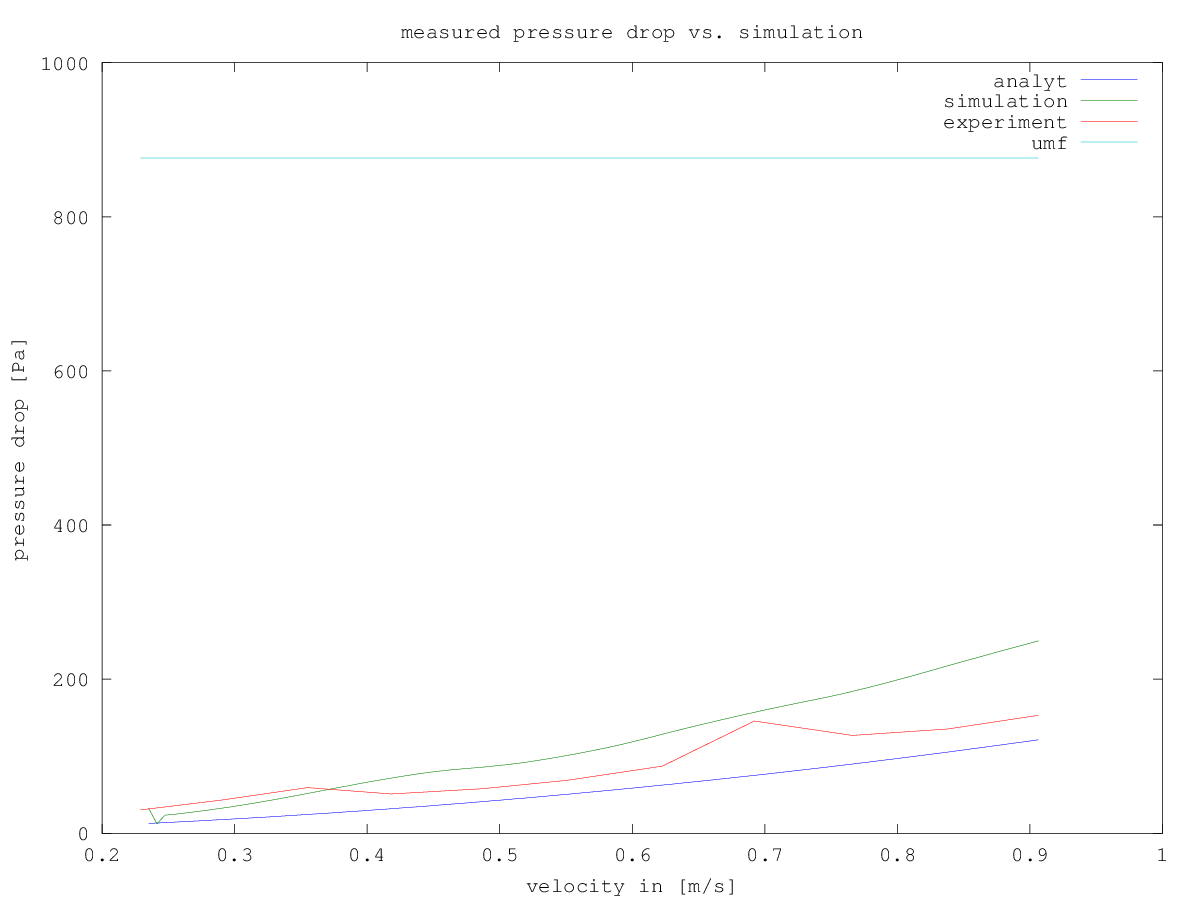
\includegraphics{009mono_glass_d2_h1300_v2_R02_xlsx_5}
\caption[pressure drop: exp-an-sim]{pressure drop: exp-an-sim: mono glass d2 h1300 v2 R02 xlsx 5}
\label{comparisonanalyticalexperimentsimulation}
\end{sidewaysfigure}

\subsection{Venturi device}
\label{subsection:venturidevice}

Initially conceived as an extension of the mass hopper flow tester, I am still stuck in the design phase and I am evaluating if dropping it completely.\\
% !TEX encoding = UTF-8
% !TEX TS-program = pdflatex
% !TEX root = ../Articolo.tex
% !TEX spellcheck = it-IT

%************************************************
\section{Behavior Investigation}
\label{section:behaviorinvestigation}
%************************************************

This is the fourth draft of what should be the main topic of my PhD Thesis. 
The \textbf{ToC} is developed accordingly and attached.

\subsection{Investigation topcis}
\label{subsection:investigationtopics}

The scientific core of my PhD Thesis will investigate the following themes:
\begin{enumerate}
\item{the influence of variations (distributions) of input parameters,}
%\item{the behavior of the different properties in real life (e.g. segregation before doing the shear cell experiment),}
\item{the influence of and poly-dispersity, i.e. the possbility to extrapolate
(e.g. given 3 different fraction distributions, with known behaviors, extrapolate 
the behavior of a fourth fraction distribution).}
\end{enumerate}

\begin{figure}[!h]
\centering
\subfloat[Regression coefficient of internal friction - polidispersity ANN]
{\label{fig:041regressionavg1}
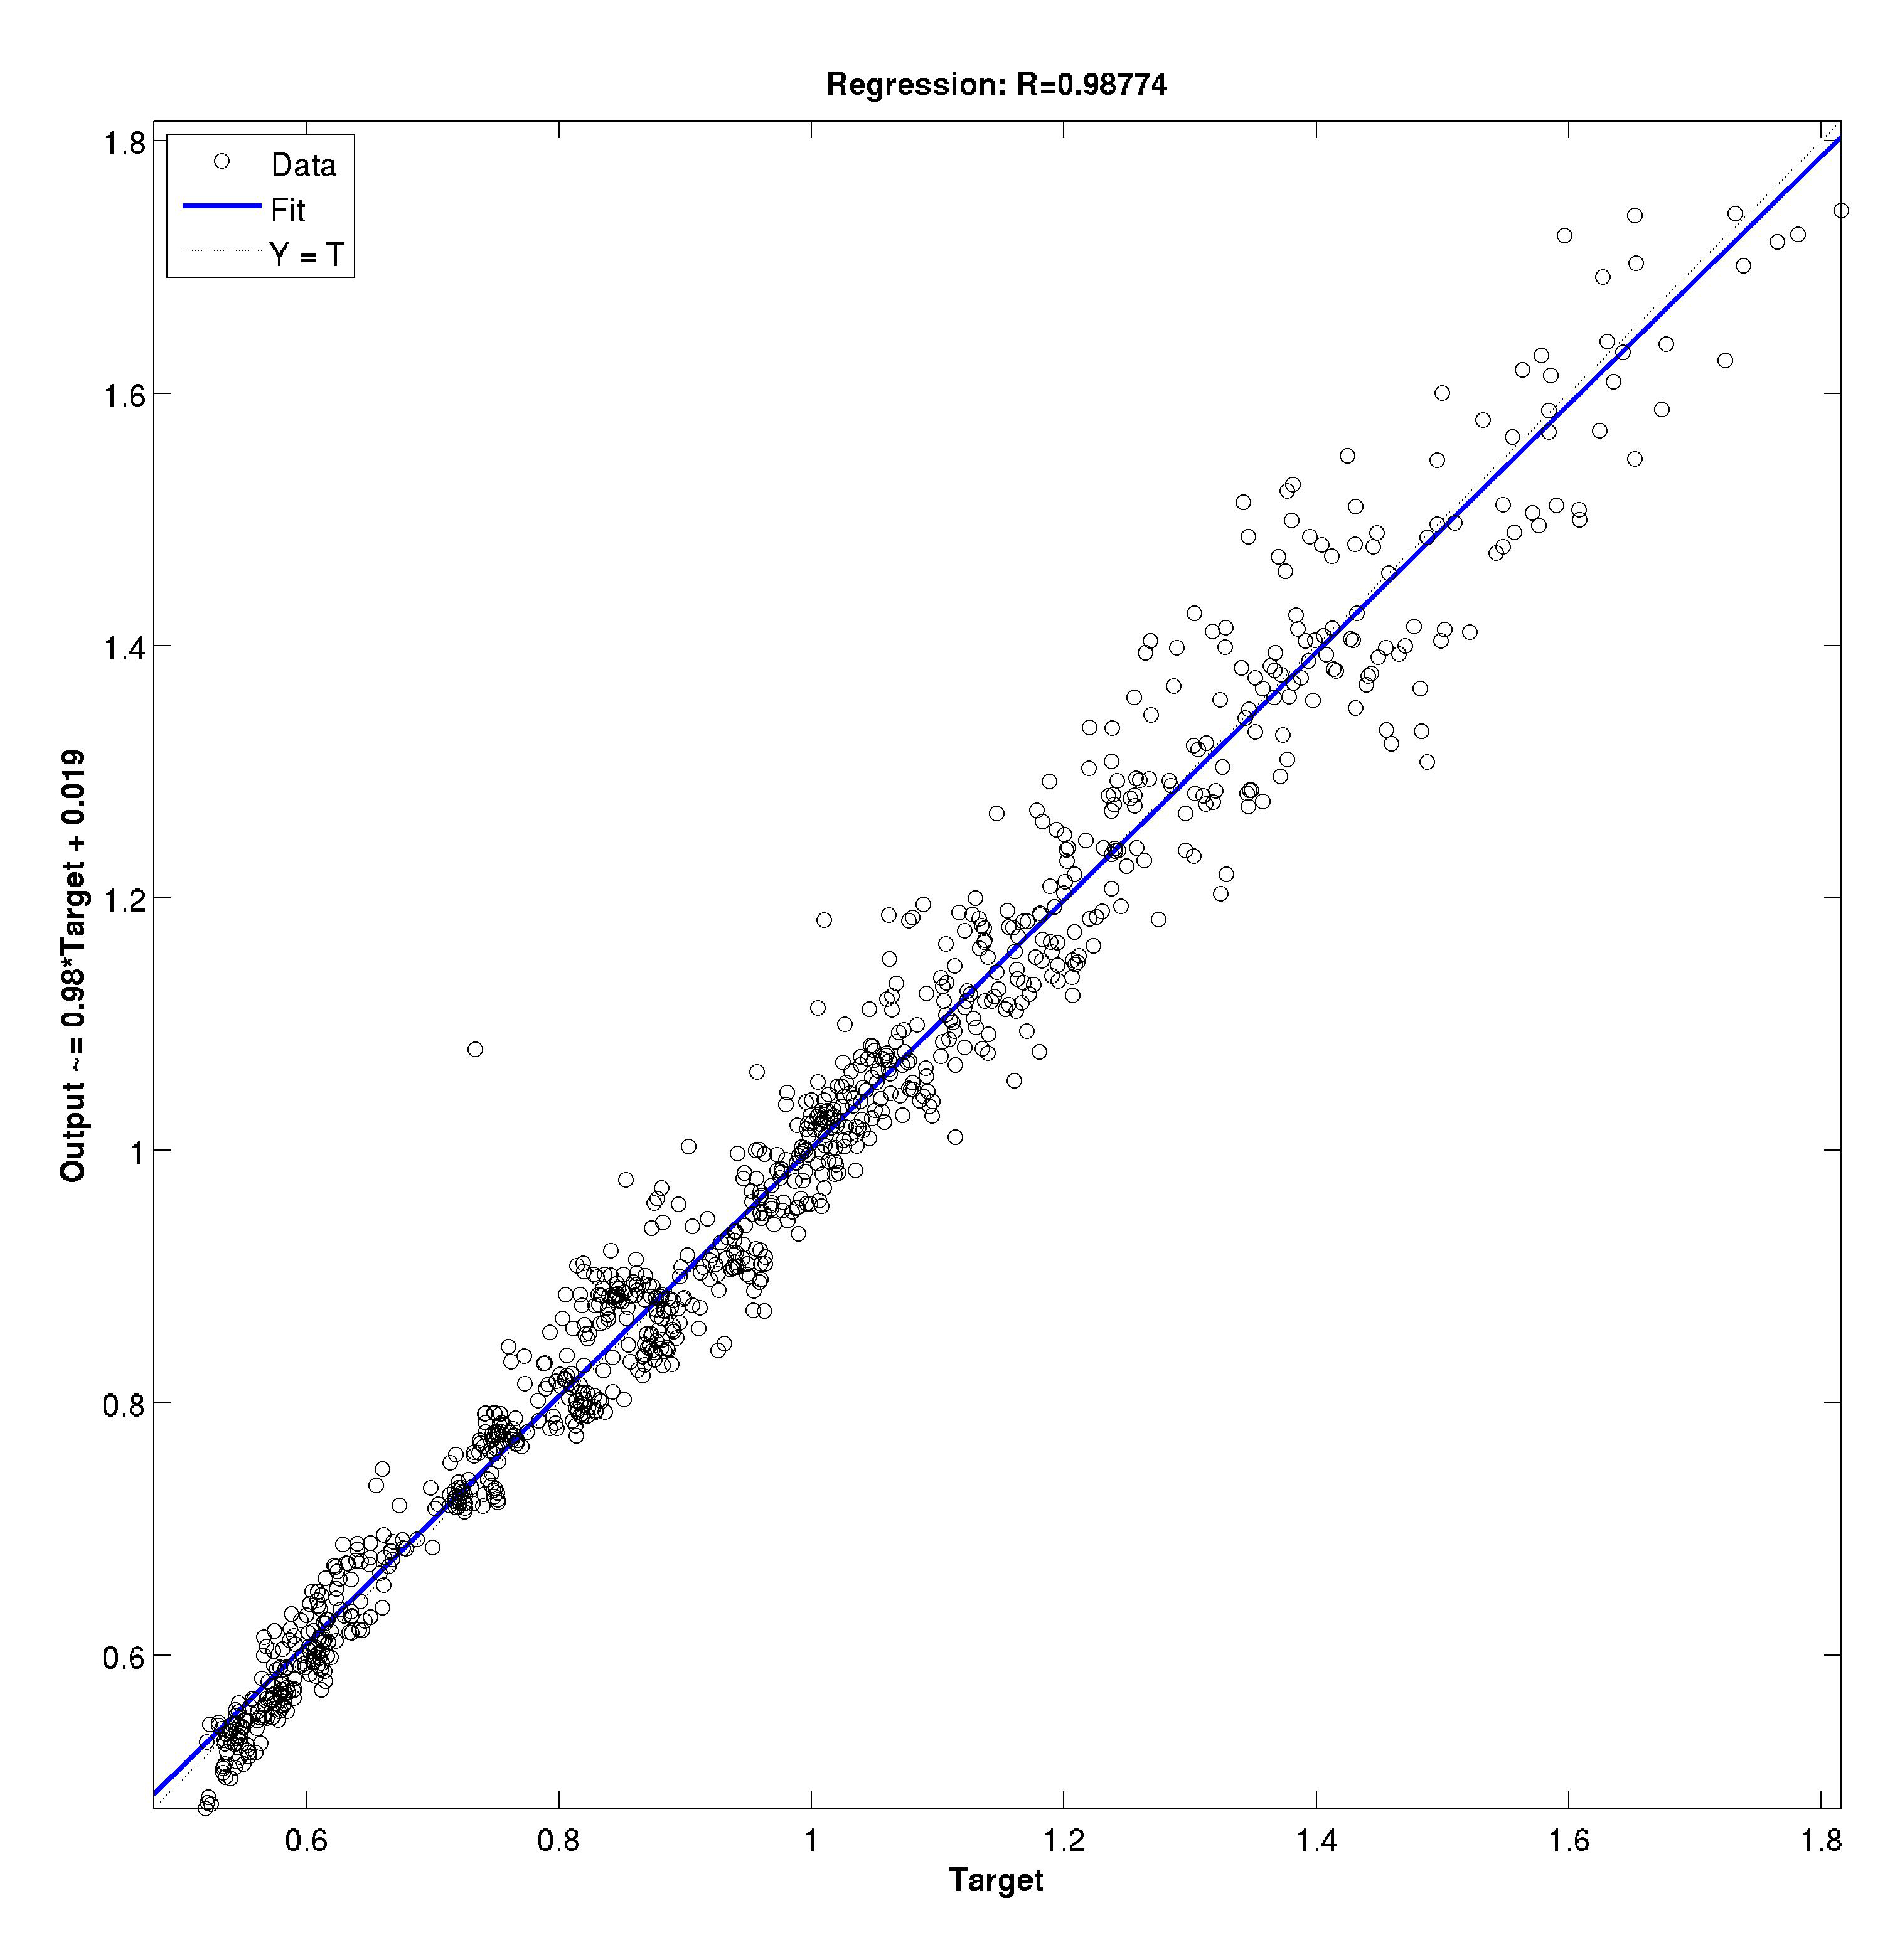
\includegraphics[width=.35\columnwidth]{041regressionavg1}} \\
\subfloat[Radius distribution with 1st simulation set]
{\label{fig:046simulationRadiusDistribution5}
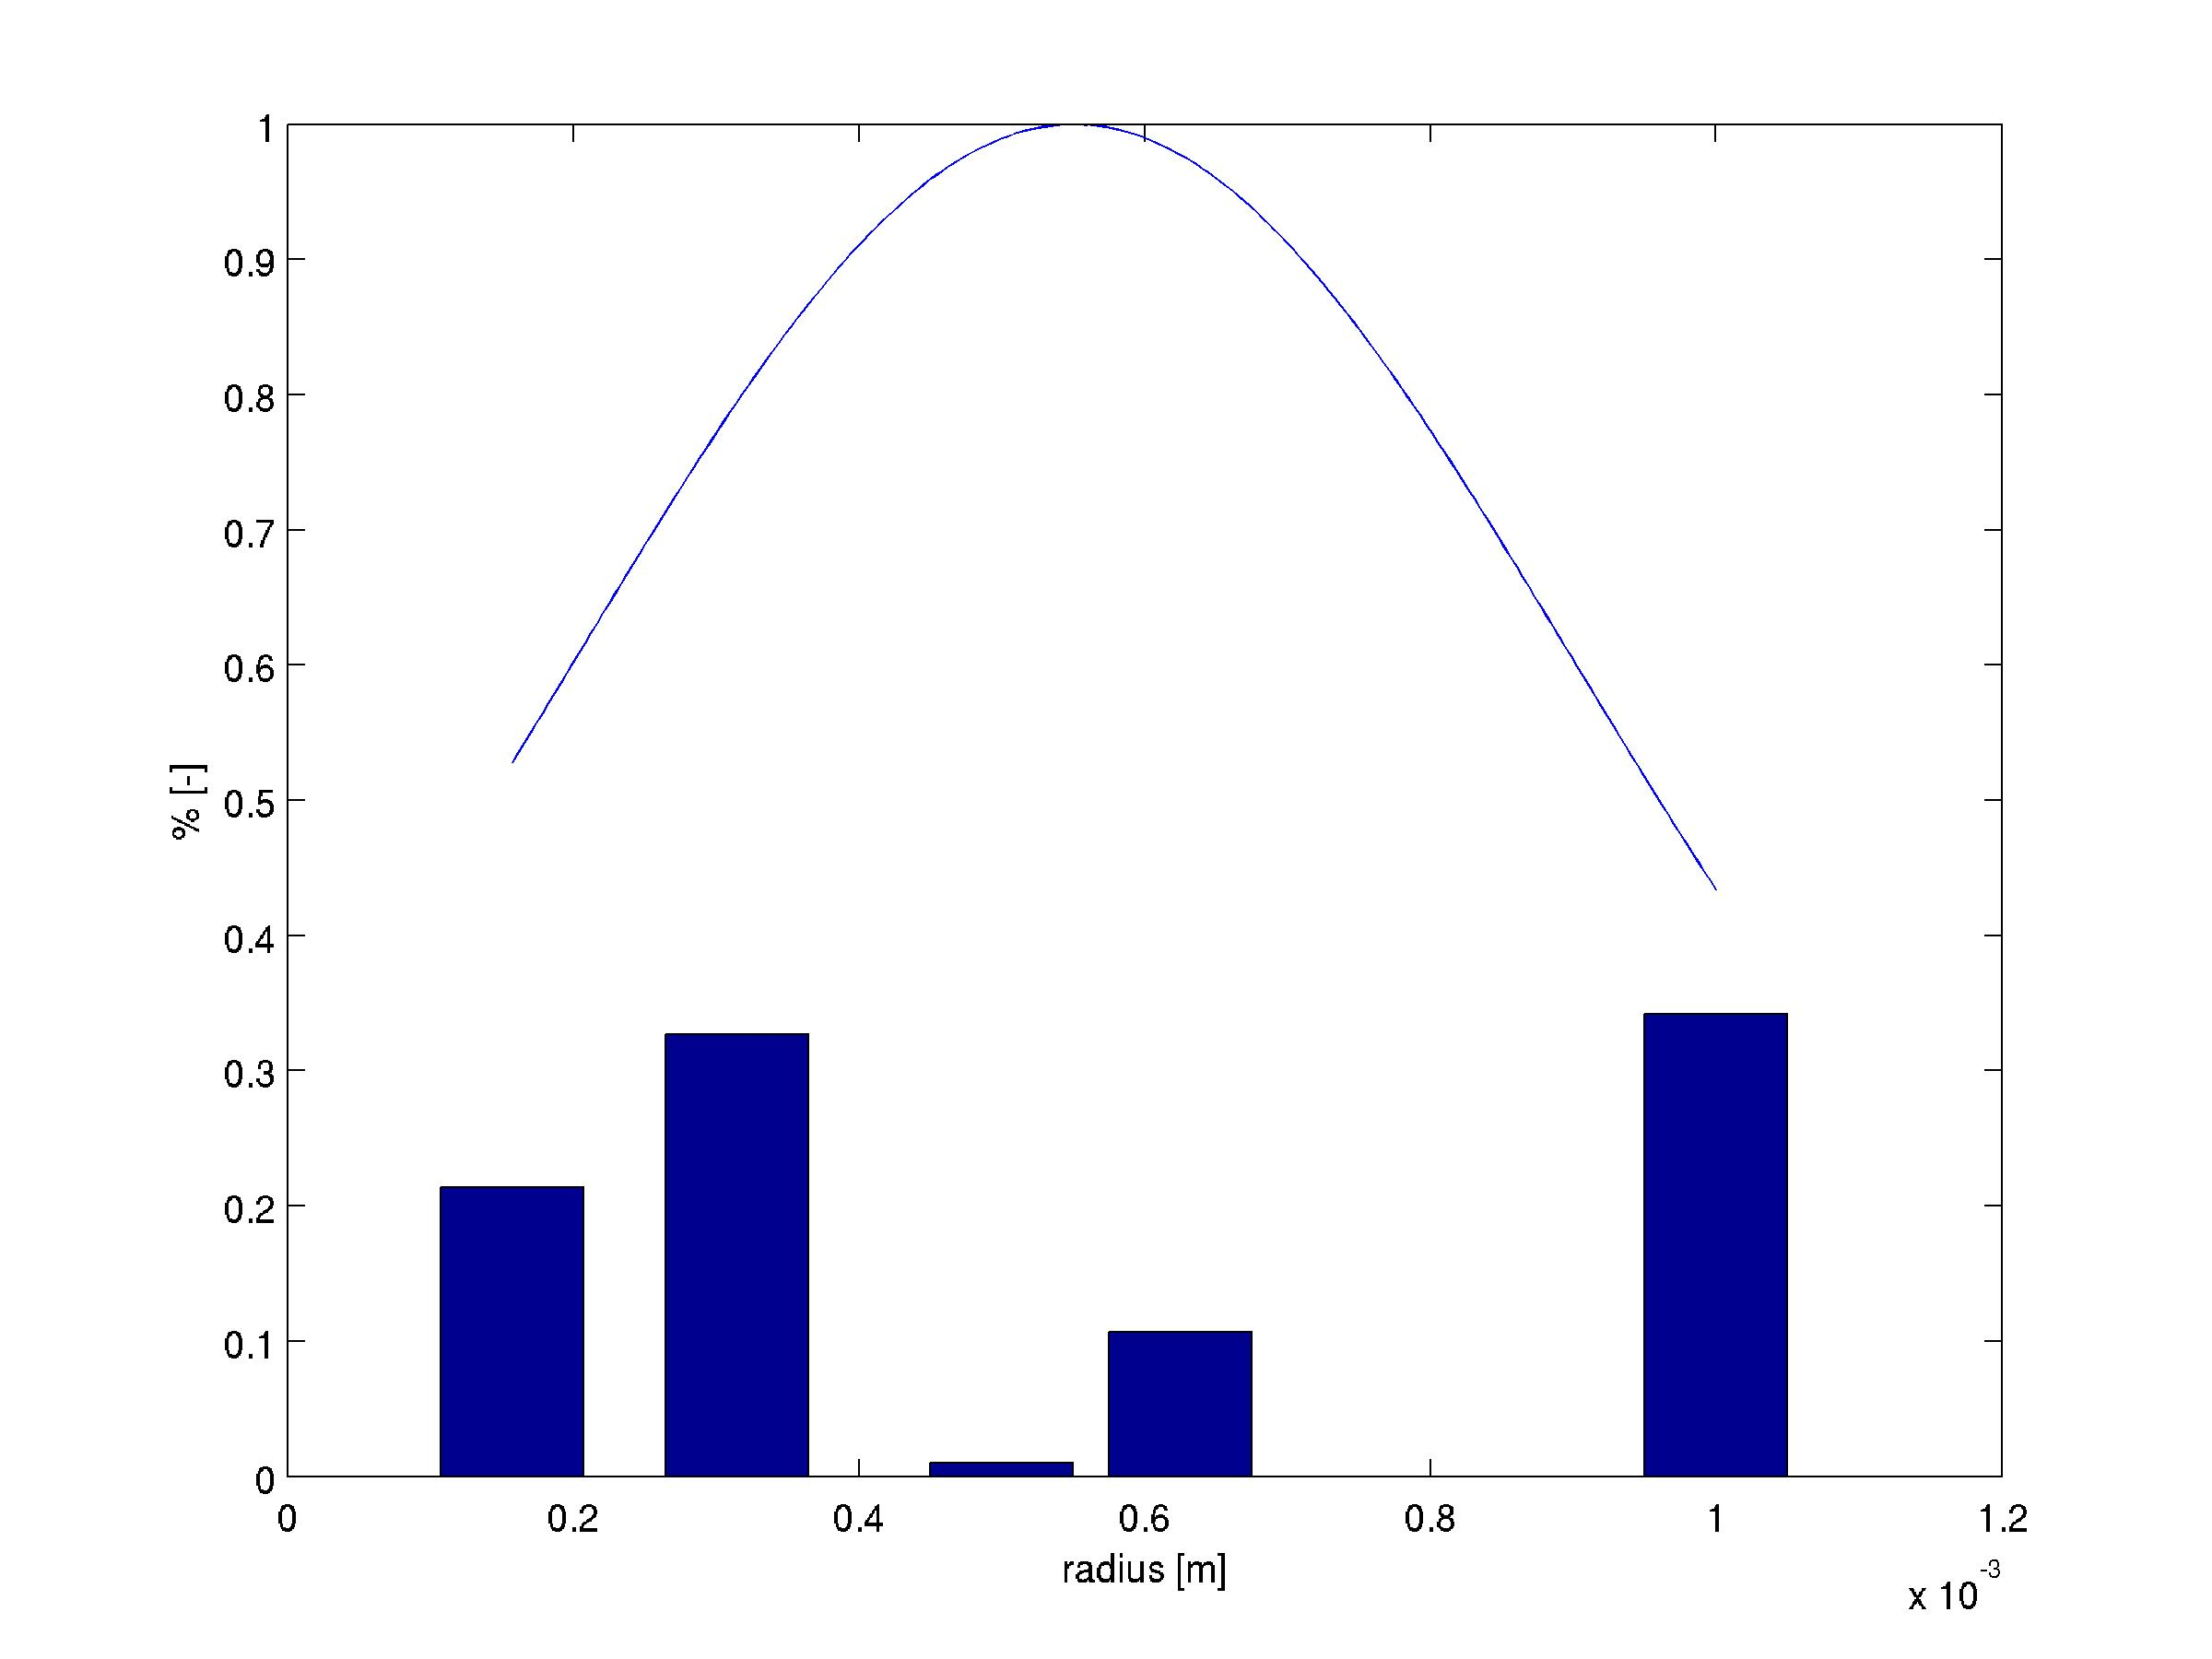
\includegraphics[width=.35\columnwidth]{046simulationRadiusDistribution5}} \quad
\subfloat[Radius distribution with 2nd simulation set]
{\label{fig:047simulationRadiusDistribution6}
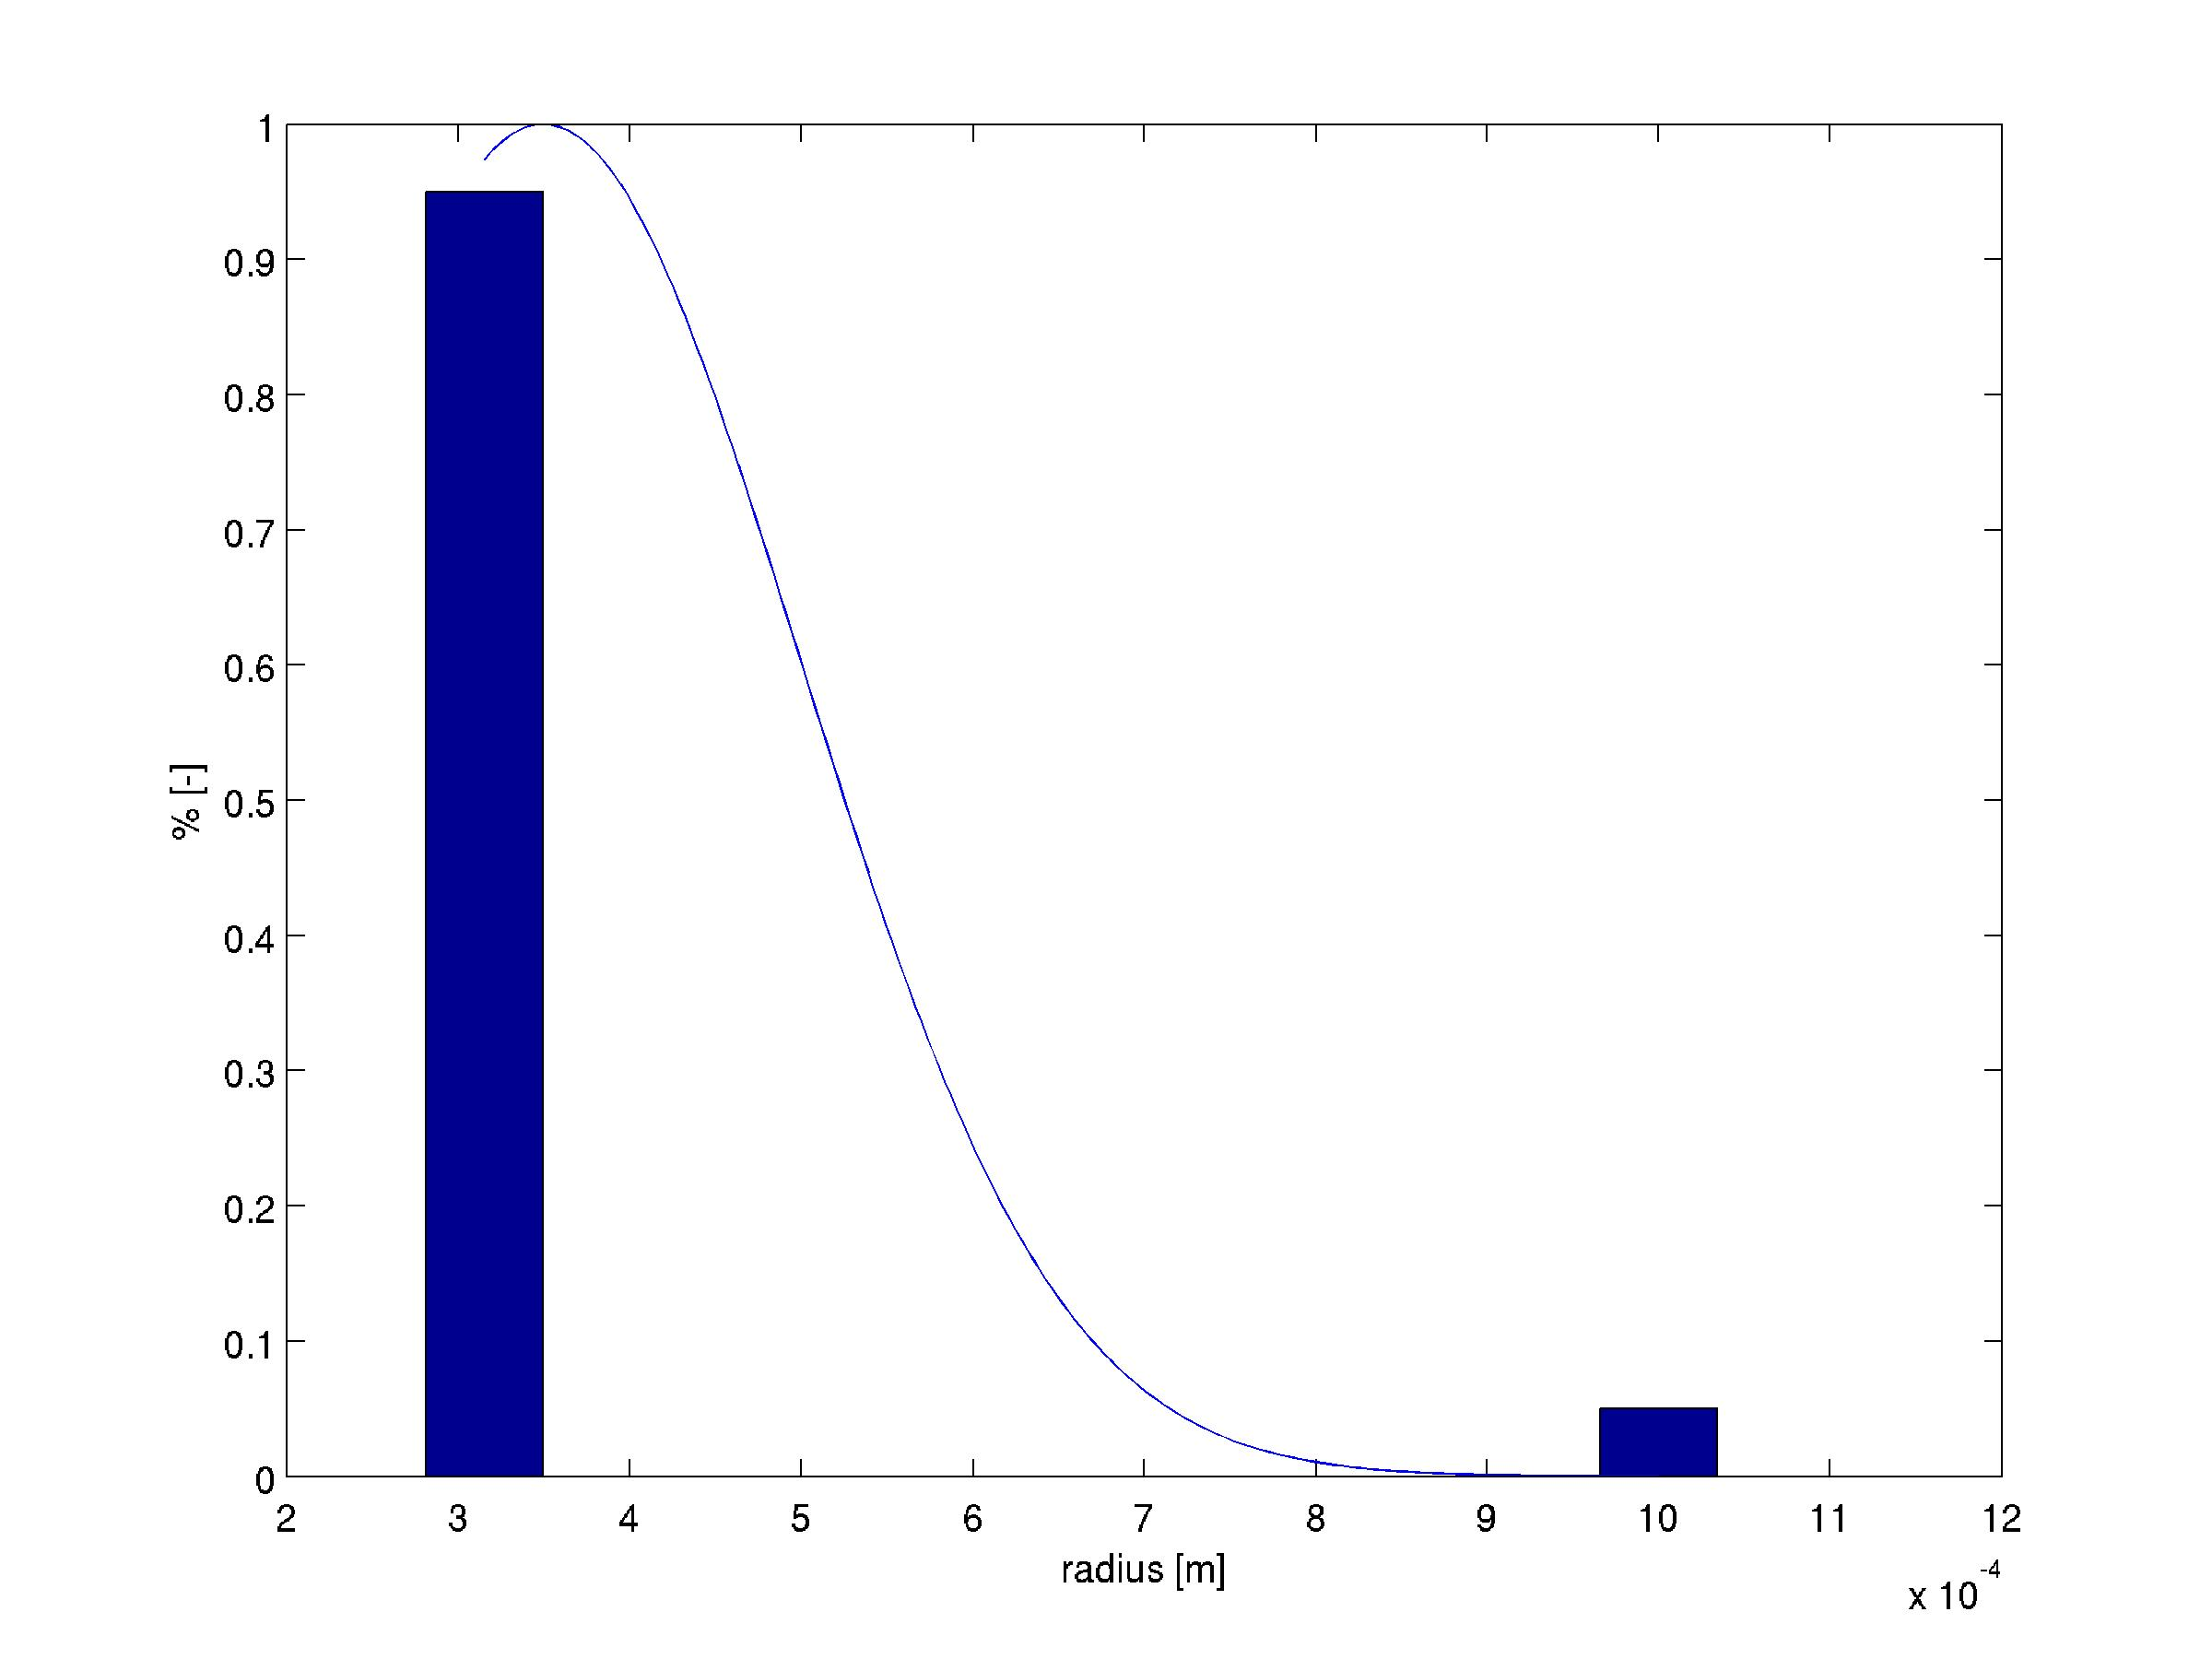
\includegraphics[width=.35\columnwidth]{047simulationRadiusDistribution6}} \\
\subfloat[Radius distribution with 3rd simulation set]
{\label{fig:048simulationRadiusDistribution7}
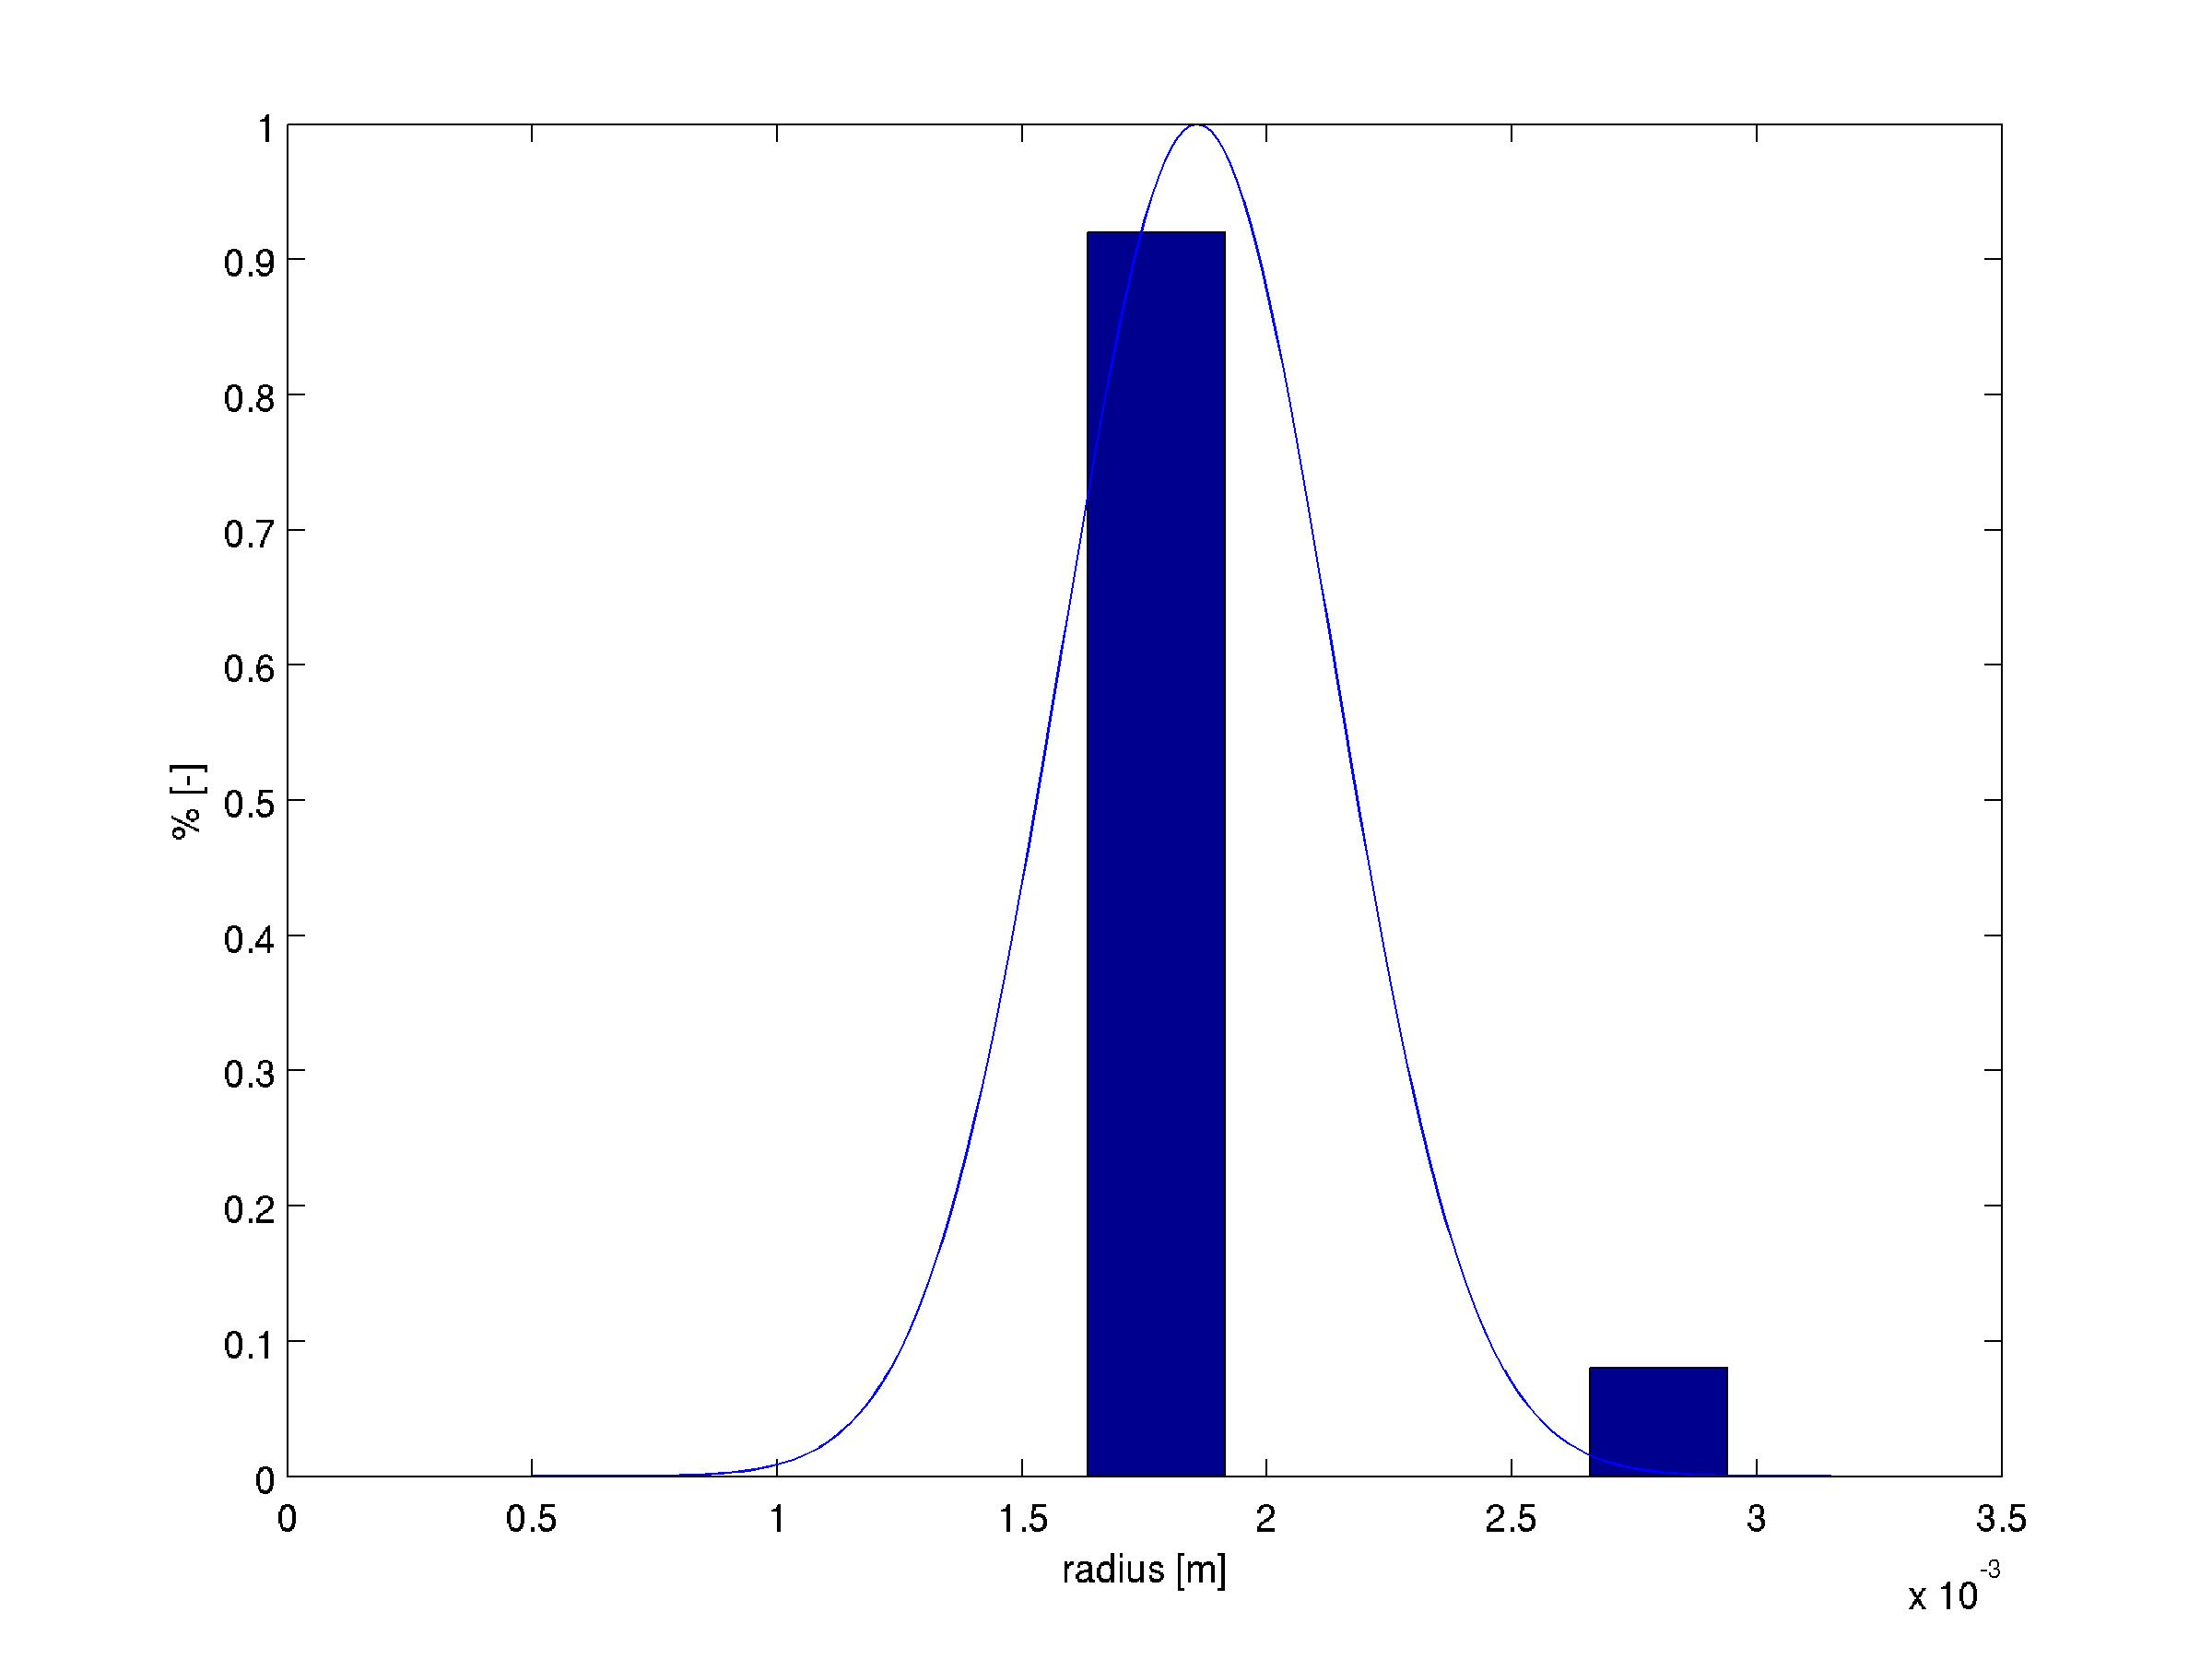
\includegraphics[width=.35\columnwidth]{048simulationRadiusDistribution7}} \quad
\subfloat[Radius distribution with 4th simulation set]
{\label{fig:049simulationRadiusDistribution8}
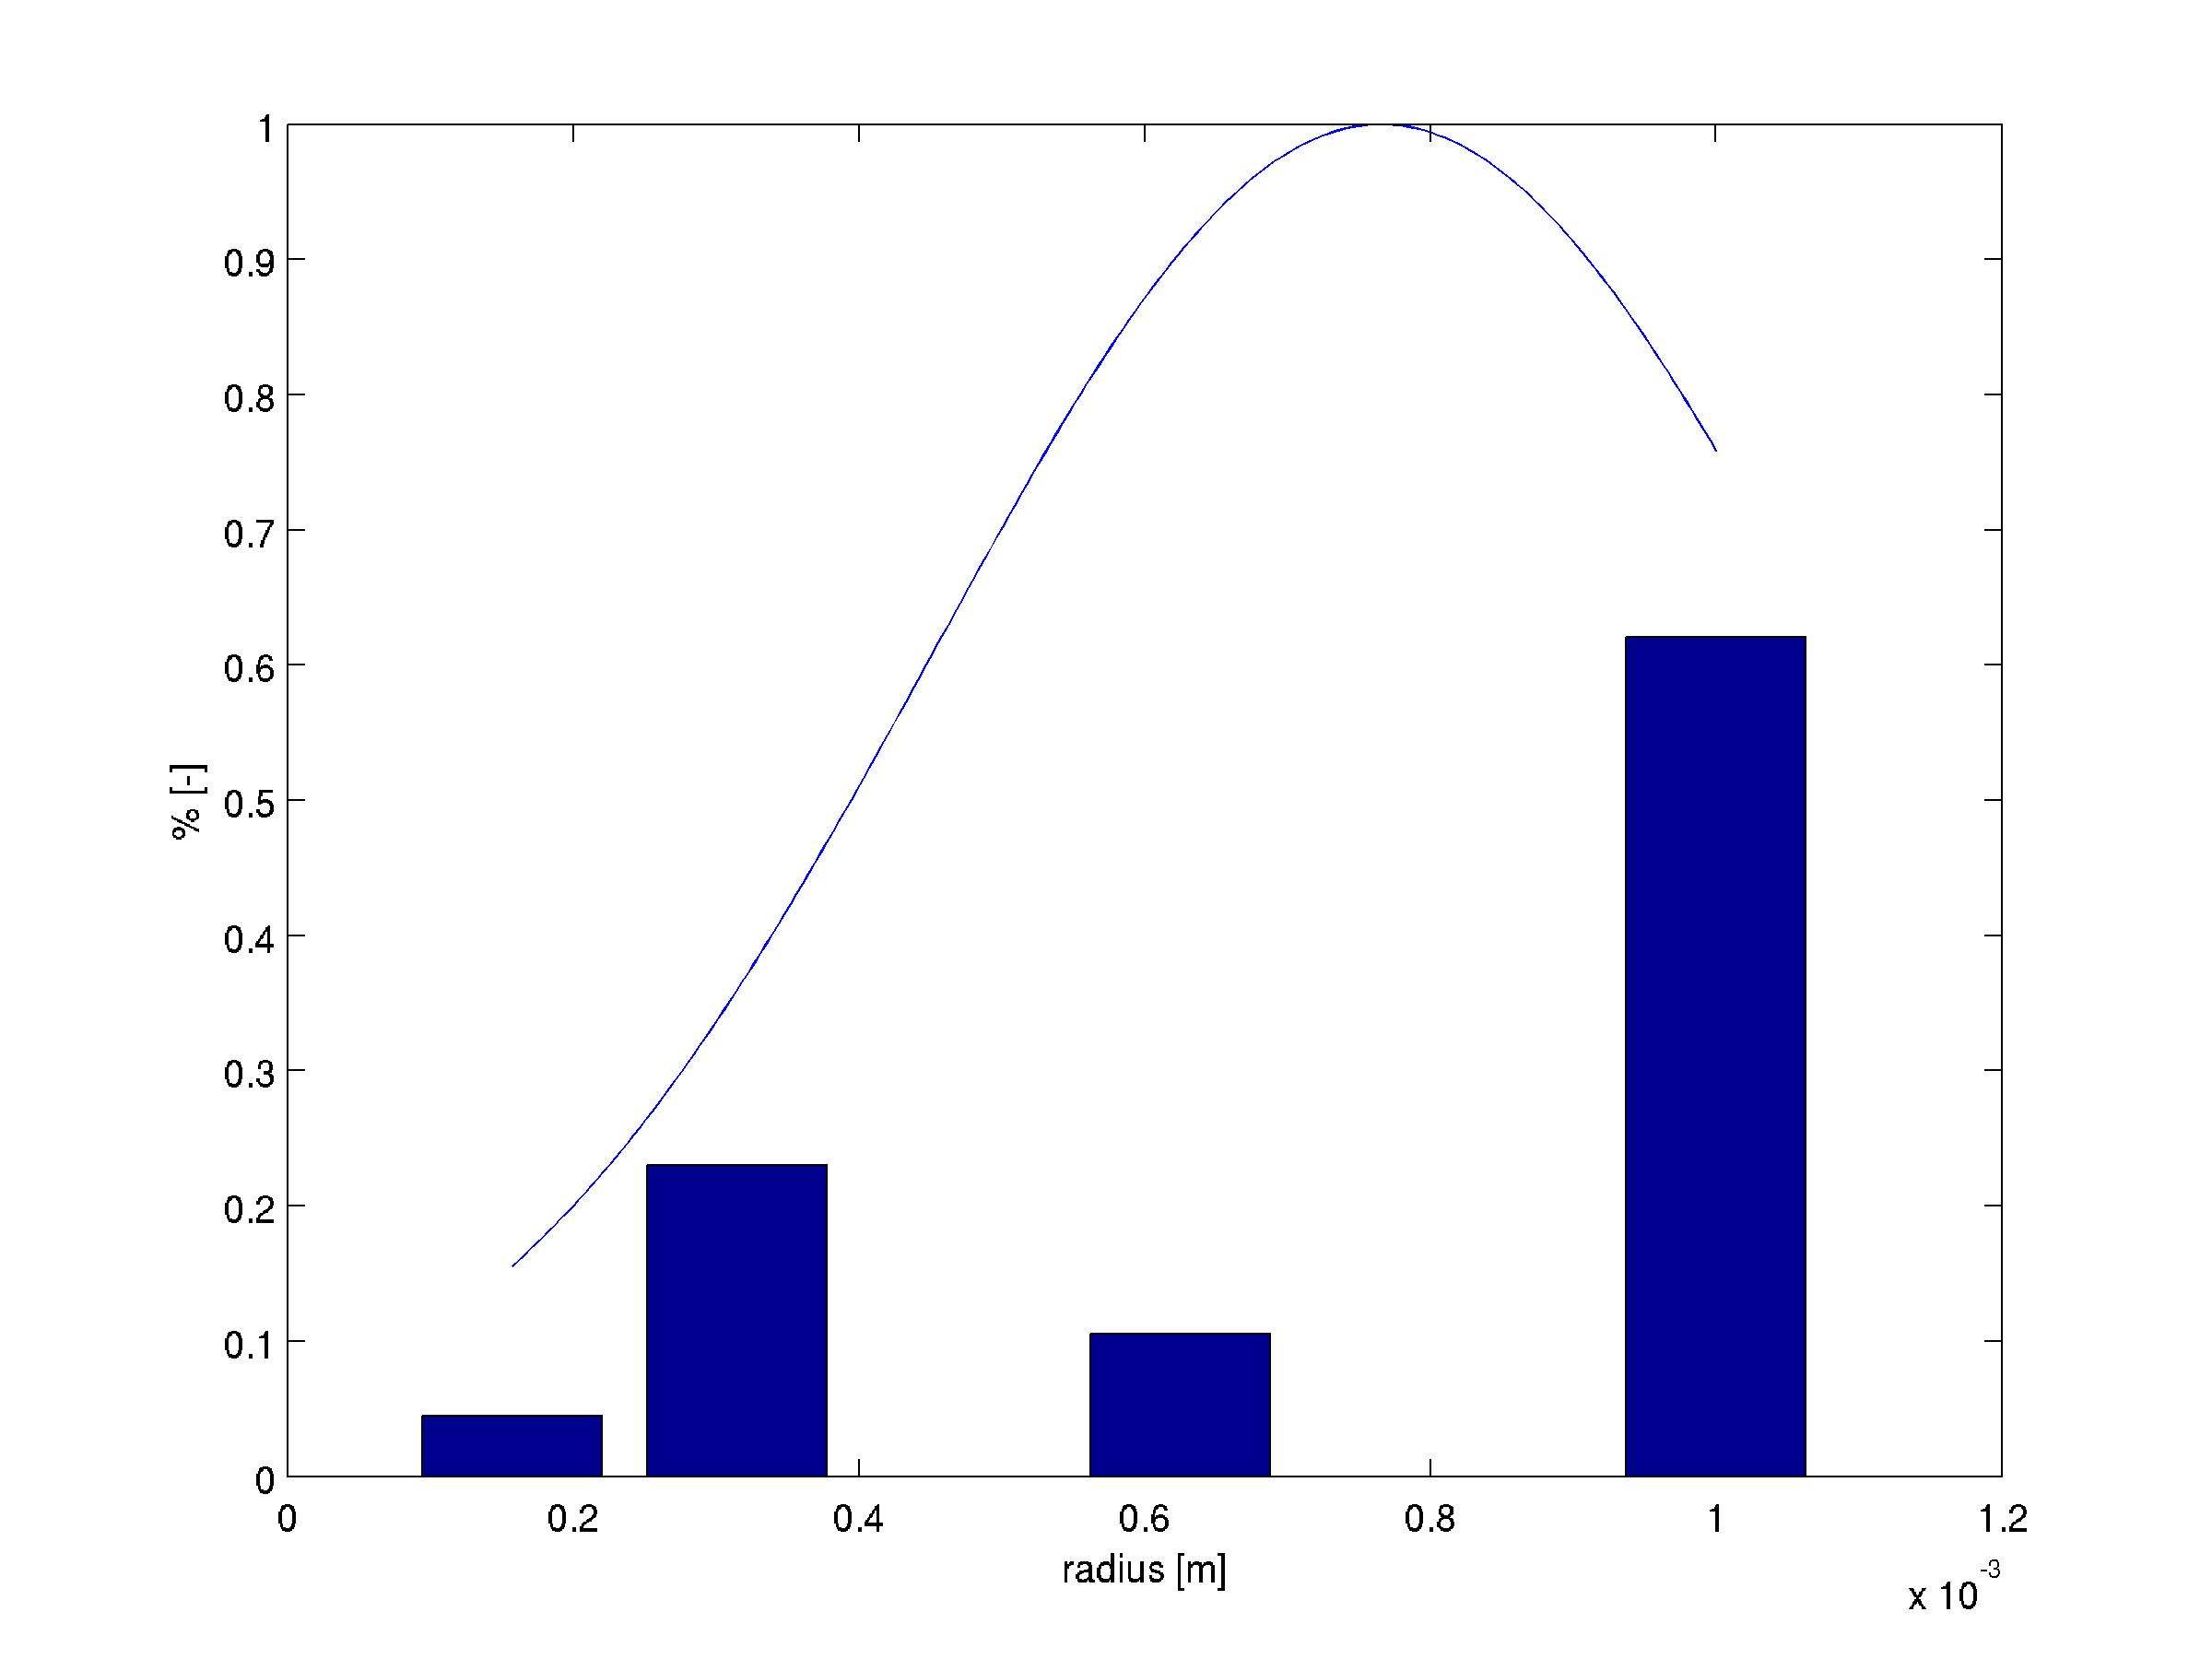
\includegraphics[width=.35\columnwidth]{049simulationRadiusDistribution8}} \\
\subfloat[Radius distribution with minimum standard deviation]
{\label{fig:042minStdDevRad}
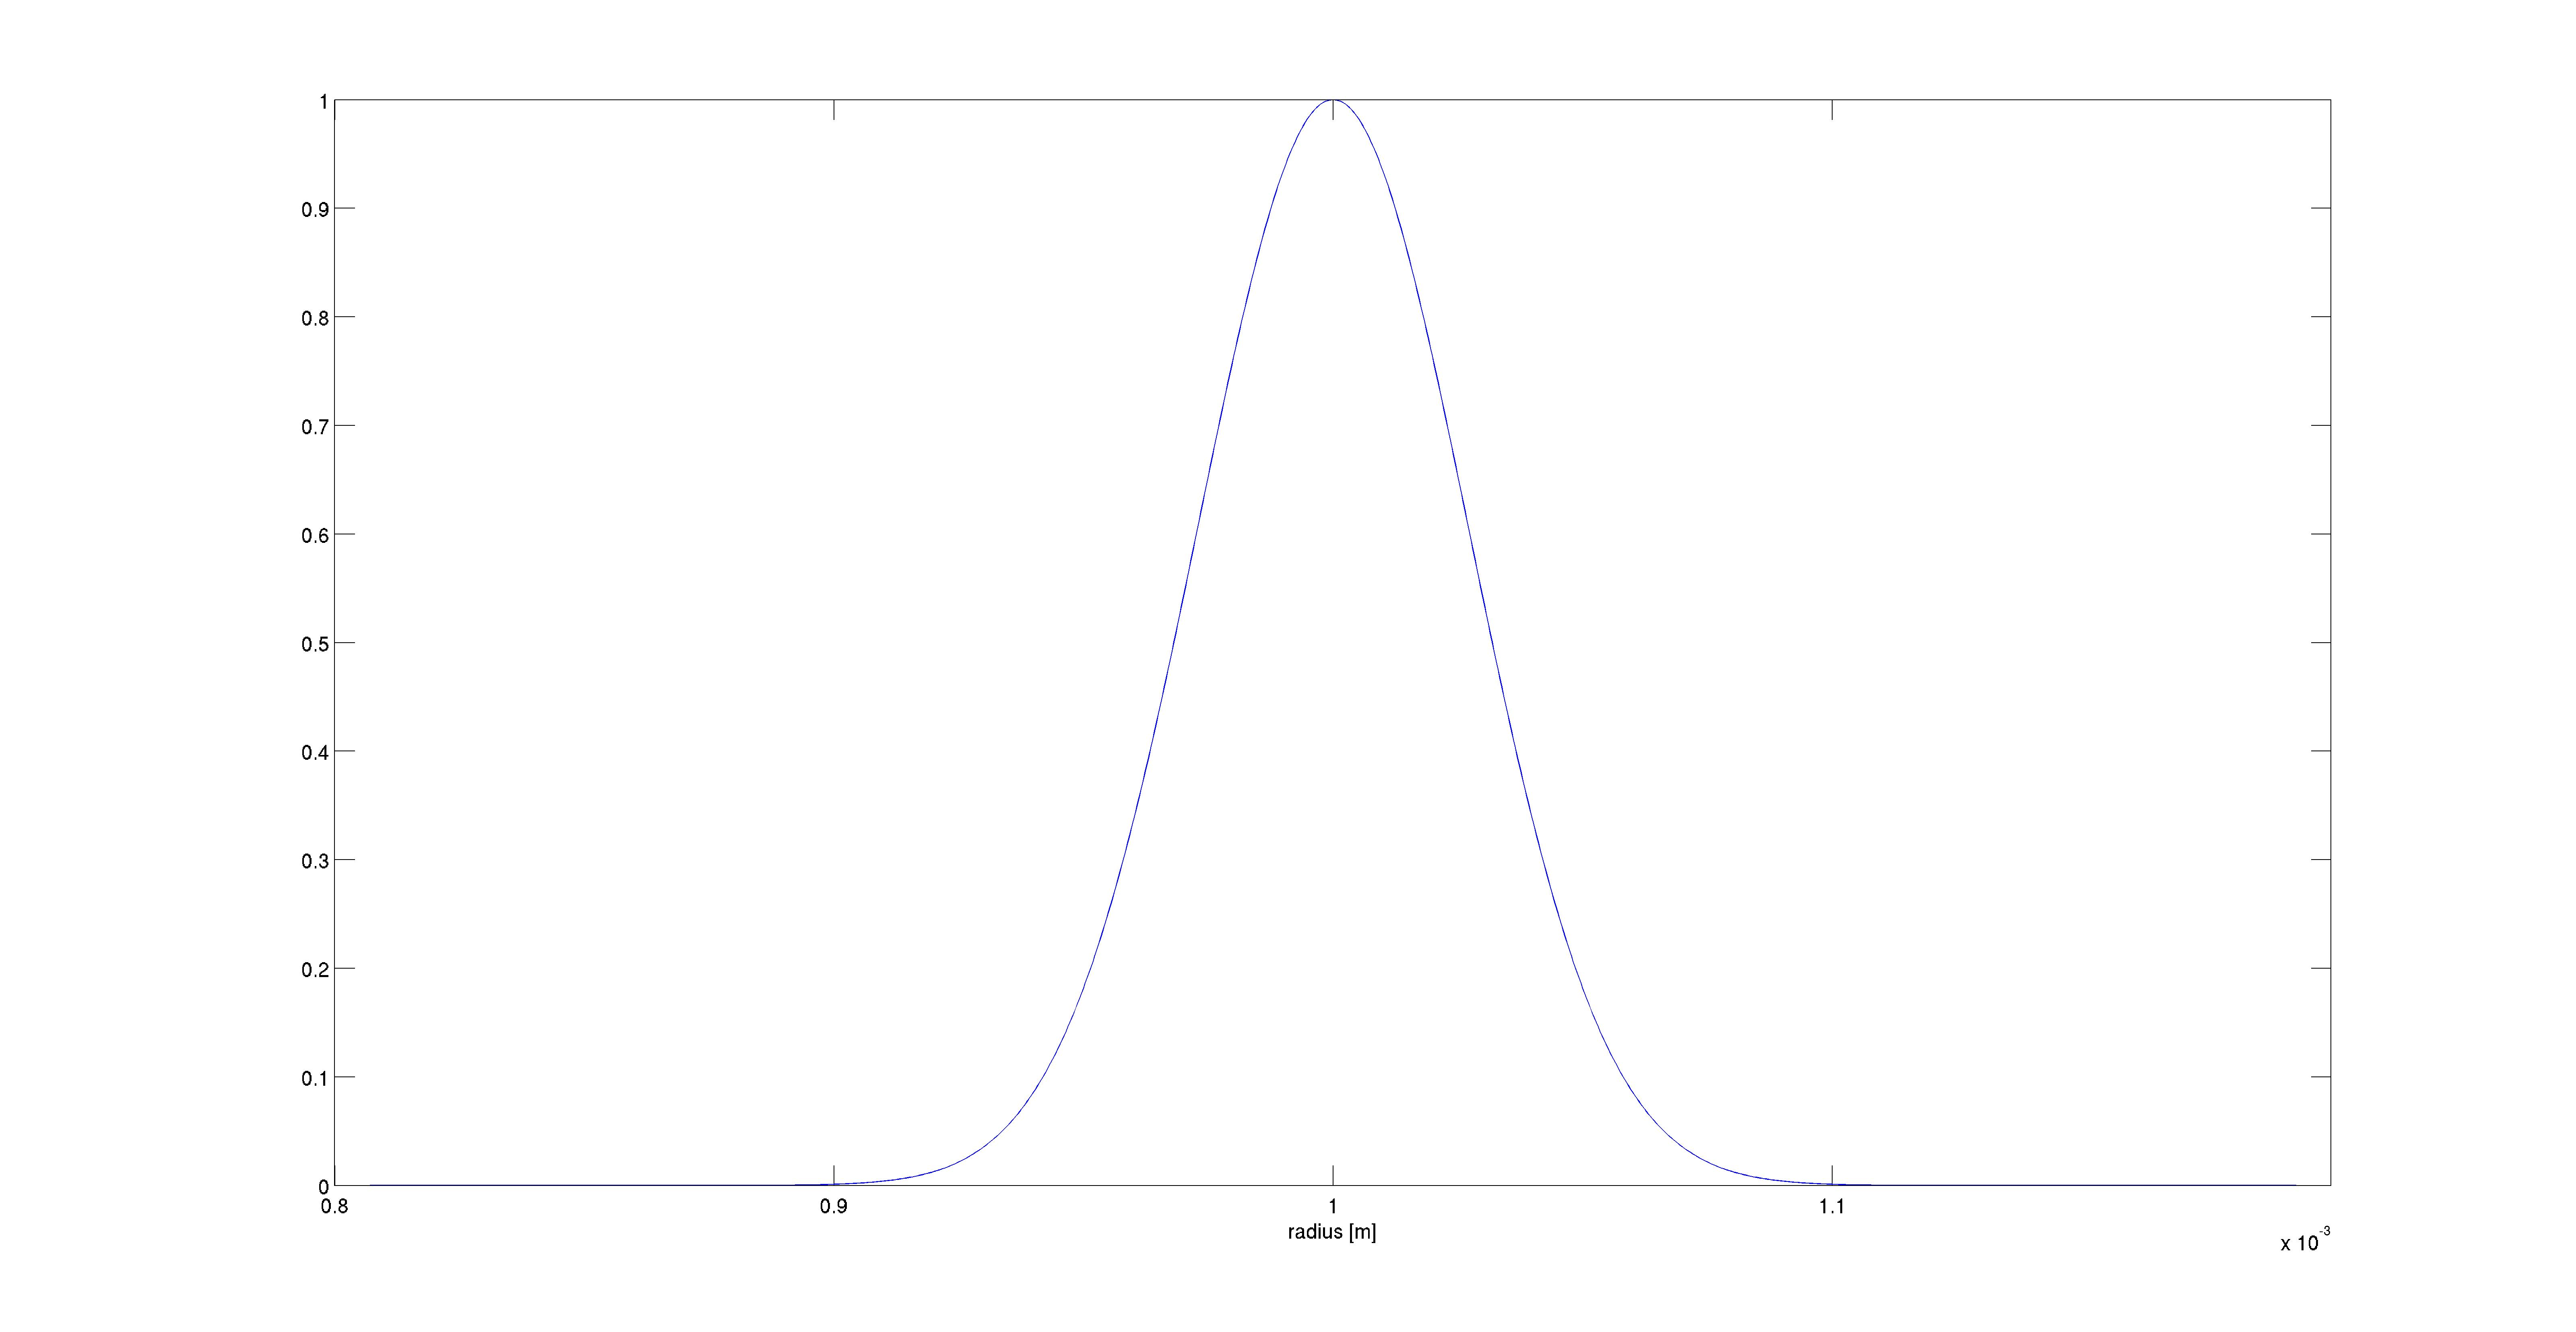
\includegraphics[width=.35\columnwidth]{042minStdDevRad}} \quad
\subfloat[Radius distribution with maximum standard deviation]
{\label{fig:043maxStdDevRad}
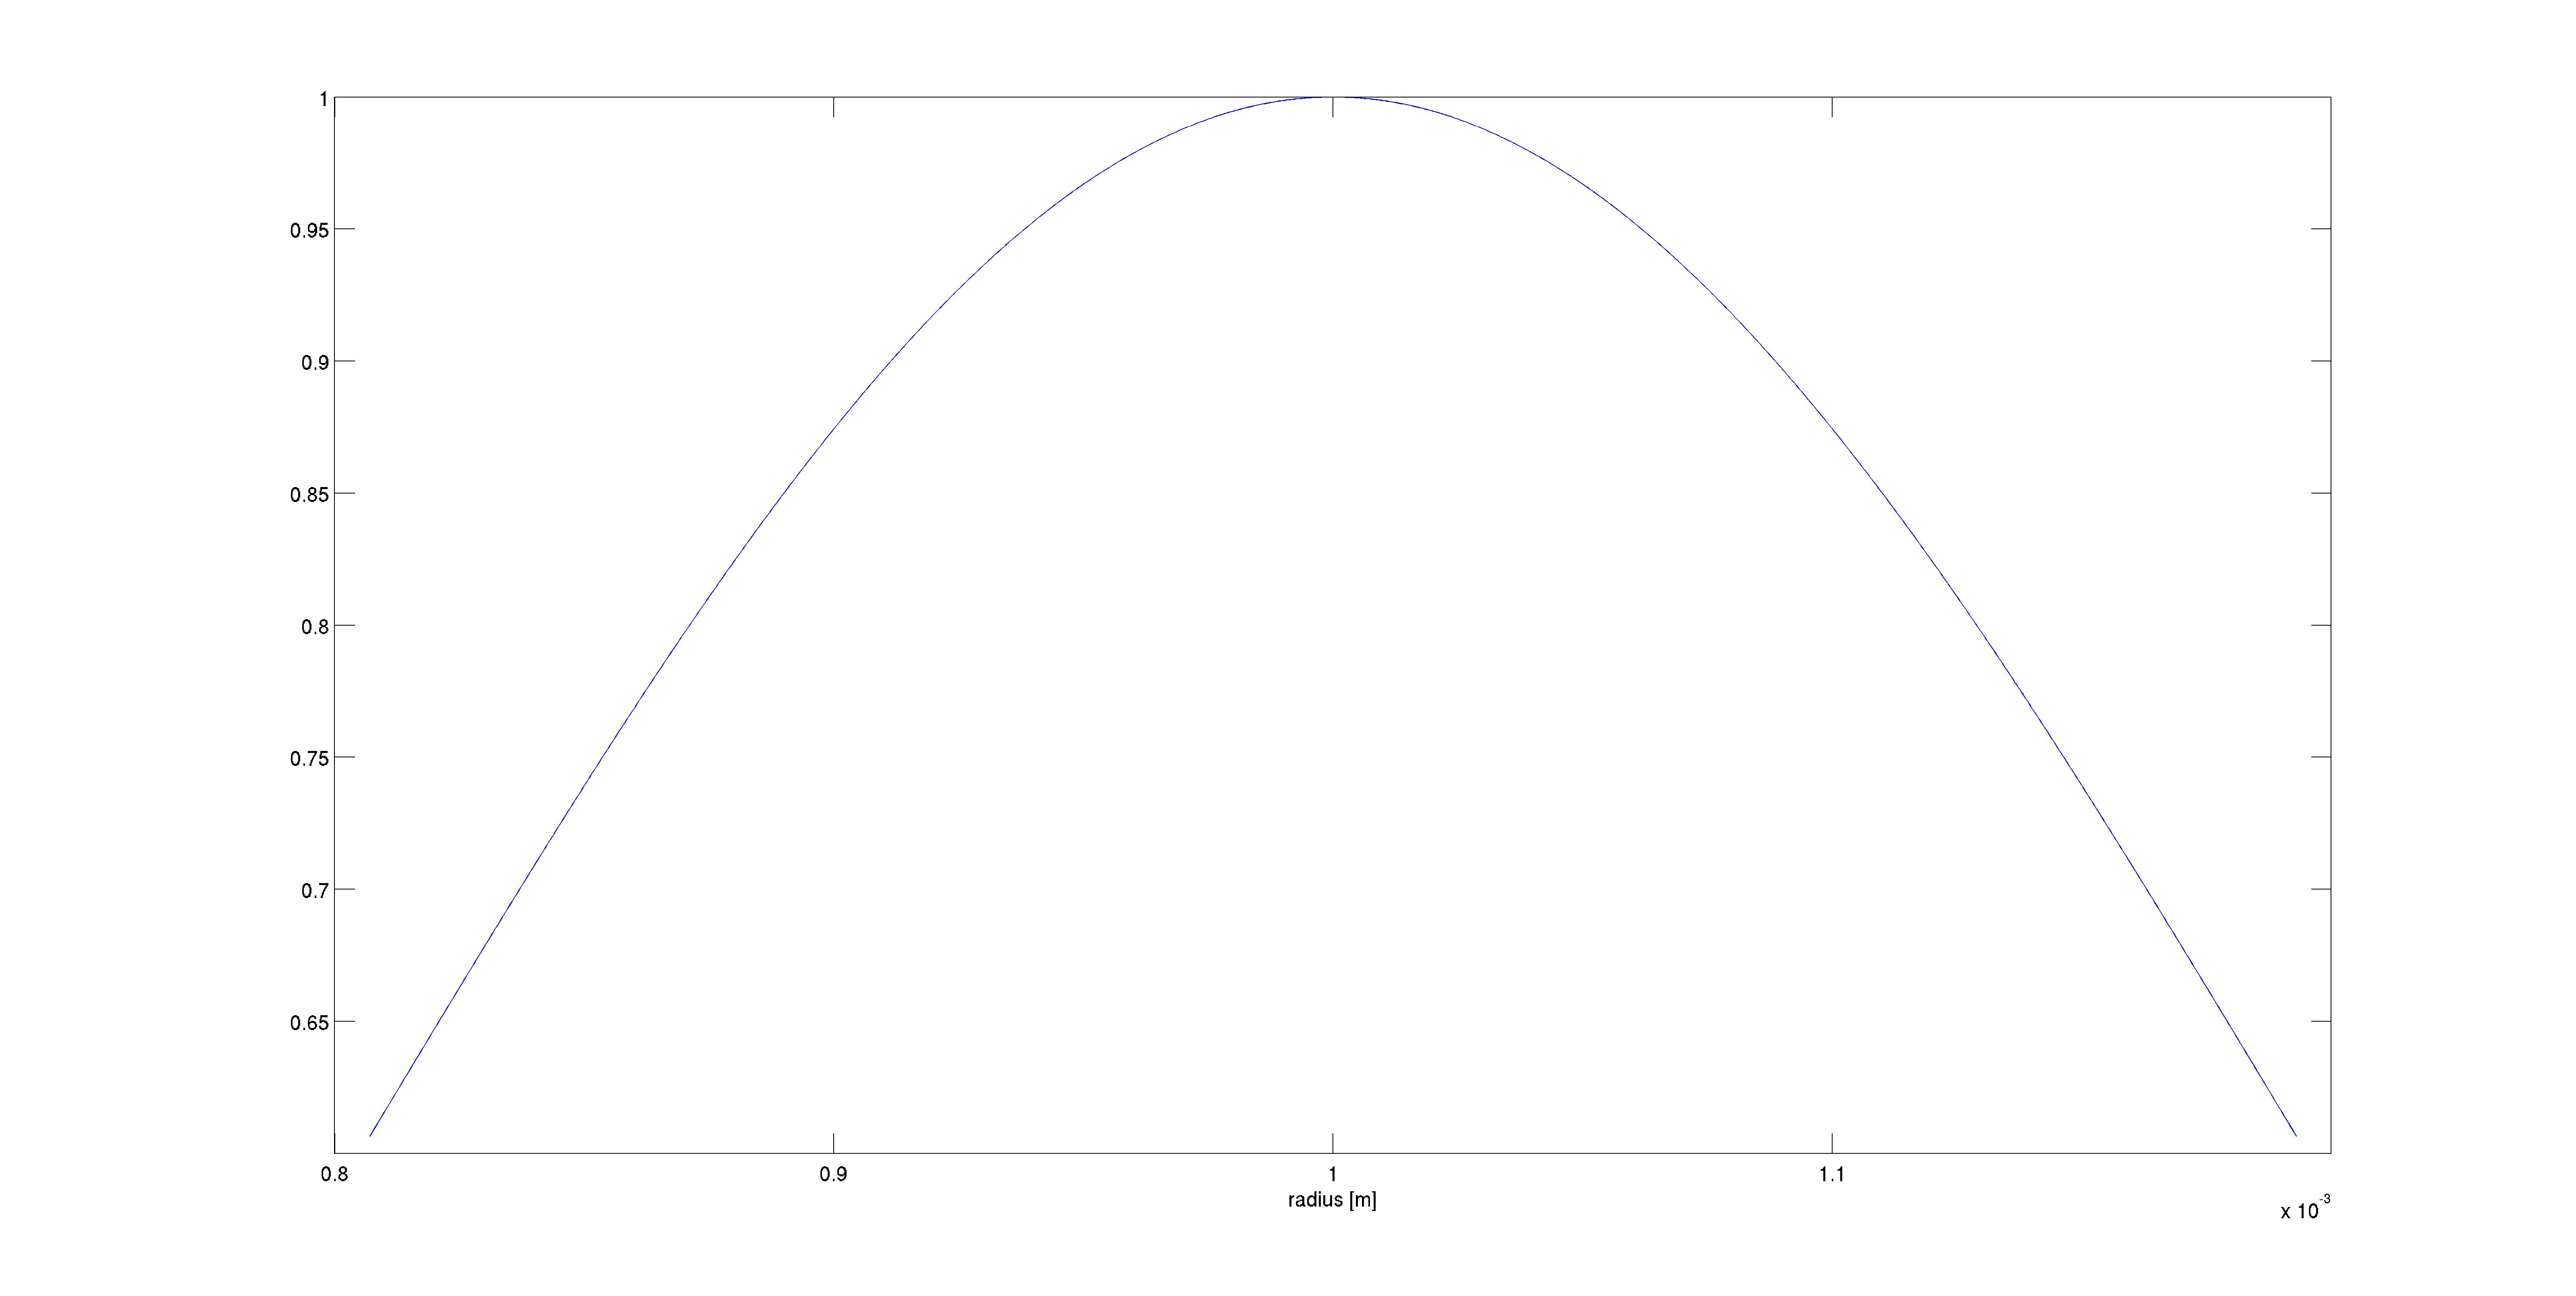
\includegraphics[width=.35\columnwidth]{043maxStdDevRad}} 
\caption[ANN and std dev radius]{ANN and std dev radius}
\label{fig:annandstddevradius}
\end{figure}

\subsection{Artificial neural network}
\label{subsection:artificialneuralnetwork}

The first core item has been completed for sinter fine with dedicated Artificial
neural networks ($ANNs$), that has been described in a journal paper draft, see
\ref{sec:elsevierpaper}.\\

I have started the second core item, I have used the polidispersity information
available (mean and standard deviation of the radius) for the simulations
already performed to train another series of $ANNs$, see Fig.
\ref{fig:annandstddevradius}.\\
Later I gave to the $ANNs$ input combinations with combinations that had a mean radius of 1 mm
and 50 different std dev, varying from 2.71e-05 m to 1.93e-04 m.
The minimum and maximum values are plotted in Fig. \ref{fig:042minStdDevRad} and
\ref{fig:043maxStdDevRad} respectively.\\
The variation of the bulk values (adimensional) against the std dev of the
radius calculated by the three $ANNs$ can be seen in Fig. \ref{fig:044bulkMean}:
the bulk density and the coefficient of internal friction after
compaction respond according to theory (more dispersion --> more small particles
--> higher compaction --> higher density and friction).
The coefficient of internal friction before compaction does not.
I am investigated this issue by creating a new, dedicated, $DEM$ simulations
set.


\begin{figure}[!h]
\centering
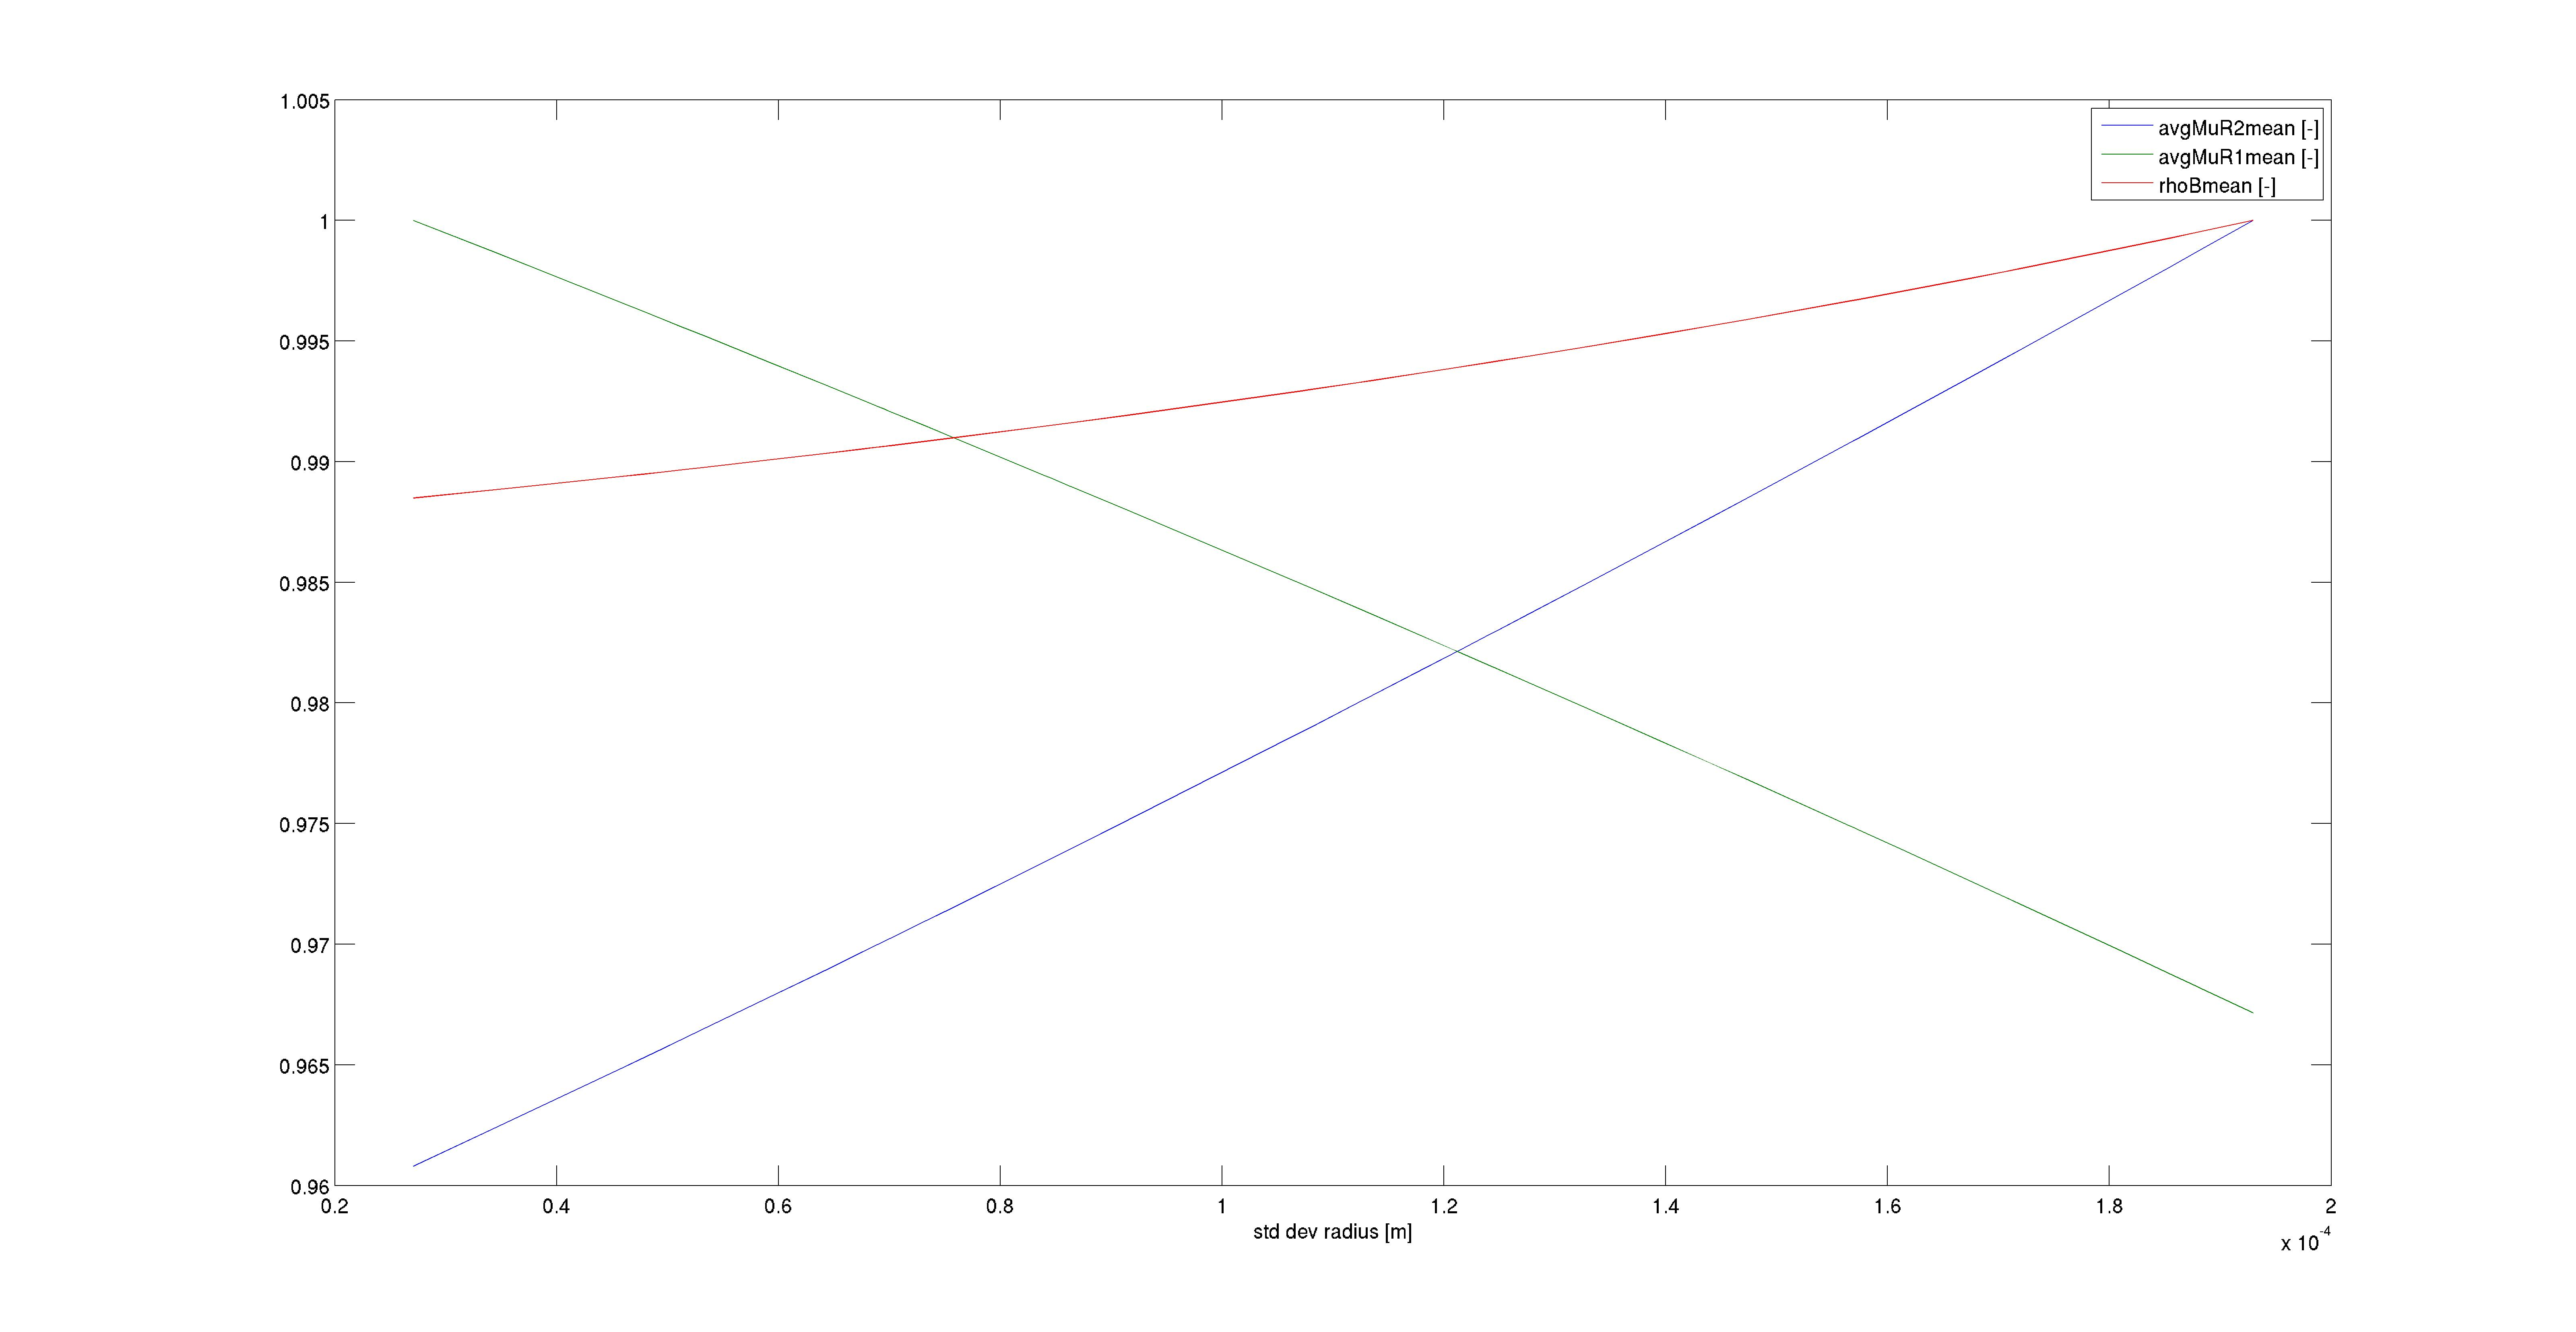
\includegraphics[width=.96\columnwidth]{044bulkMean}
\caption{Variation of bulk values }
\label{fig:044bulkMean}
\end{figure}

\newpage

% !TEX encoding = UTF-8
% !TEX TS-program = pdflatex
% !TEX root = ../Articolo.tex
% !TEX spellcheck = it-IT

%************************************************
\section{Elsevier Paper}
\label{sec:elsevierpaper}
%************************************************

The paper for Powder Technology has been revised.
An improved version, implementing the reviewers comments, has been submitted
June the $22^{nd}$.
It can be found in the Publications folder.\\

%% !TEX encoding = UTF-8
% !TEX TS-program = pdflatex
% !TEX root = ../Articolo.tex
% !TEX spellcheck = it-IT

%************************************************
\section{DEM Characterization Workflow Powder}
\label{section:Demcharacterizationworkflowpowder}
%************************************************

The powder characterization has not been exstensively studied yet in our lab (at least my knowledge).
Just a prototype of colliding hollow sphere was conceived, but the results had not been analyzed nor evaluated.\\

\subsection{Hollow spheres}
\label{subsection:hollowspheres}

The experimental apparatus can be seen in Figure \ref{fig:007hollowspheredevice2}. The main components are two twin aluminum spheres, independently connected via U-shaped steel structures to rotating beams. The rotation of the beams, and so the angular speed of the spheres, is registered by a couple of angle-meters.\\
The spheres are hollow, particles can be inserted inside, and the \ac{ra} is 50 millimeters.\\

\begin{figure}[!h]
\centering
\subfloat[HS experimental device]
{\label{fig:007hollowspheredevice2}%
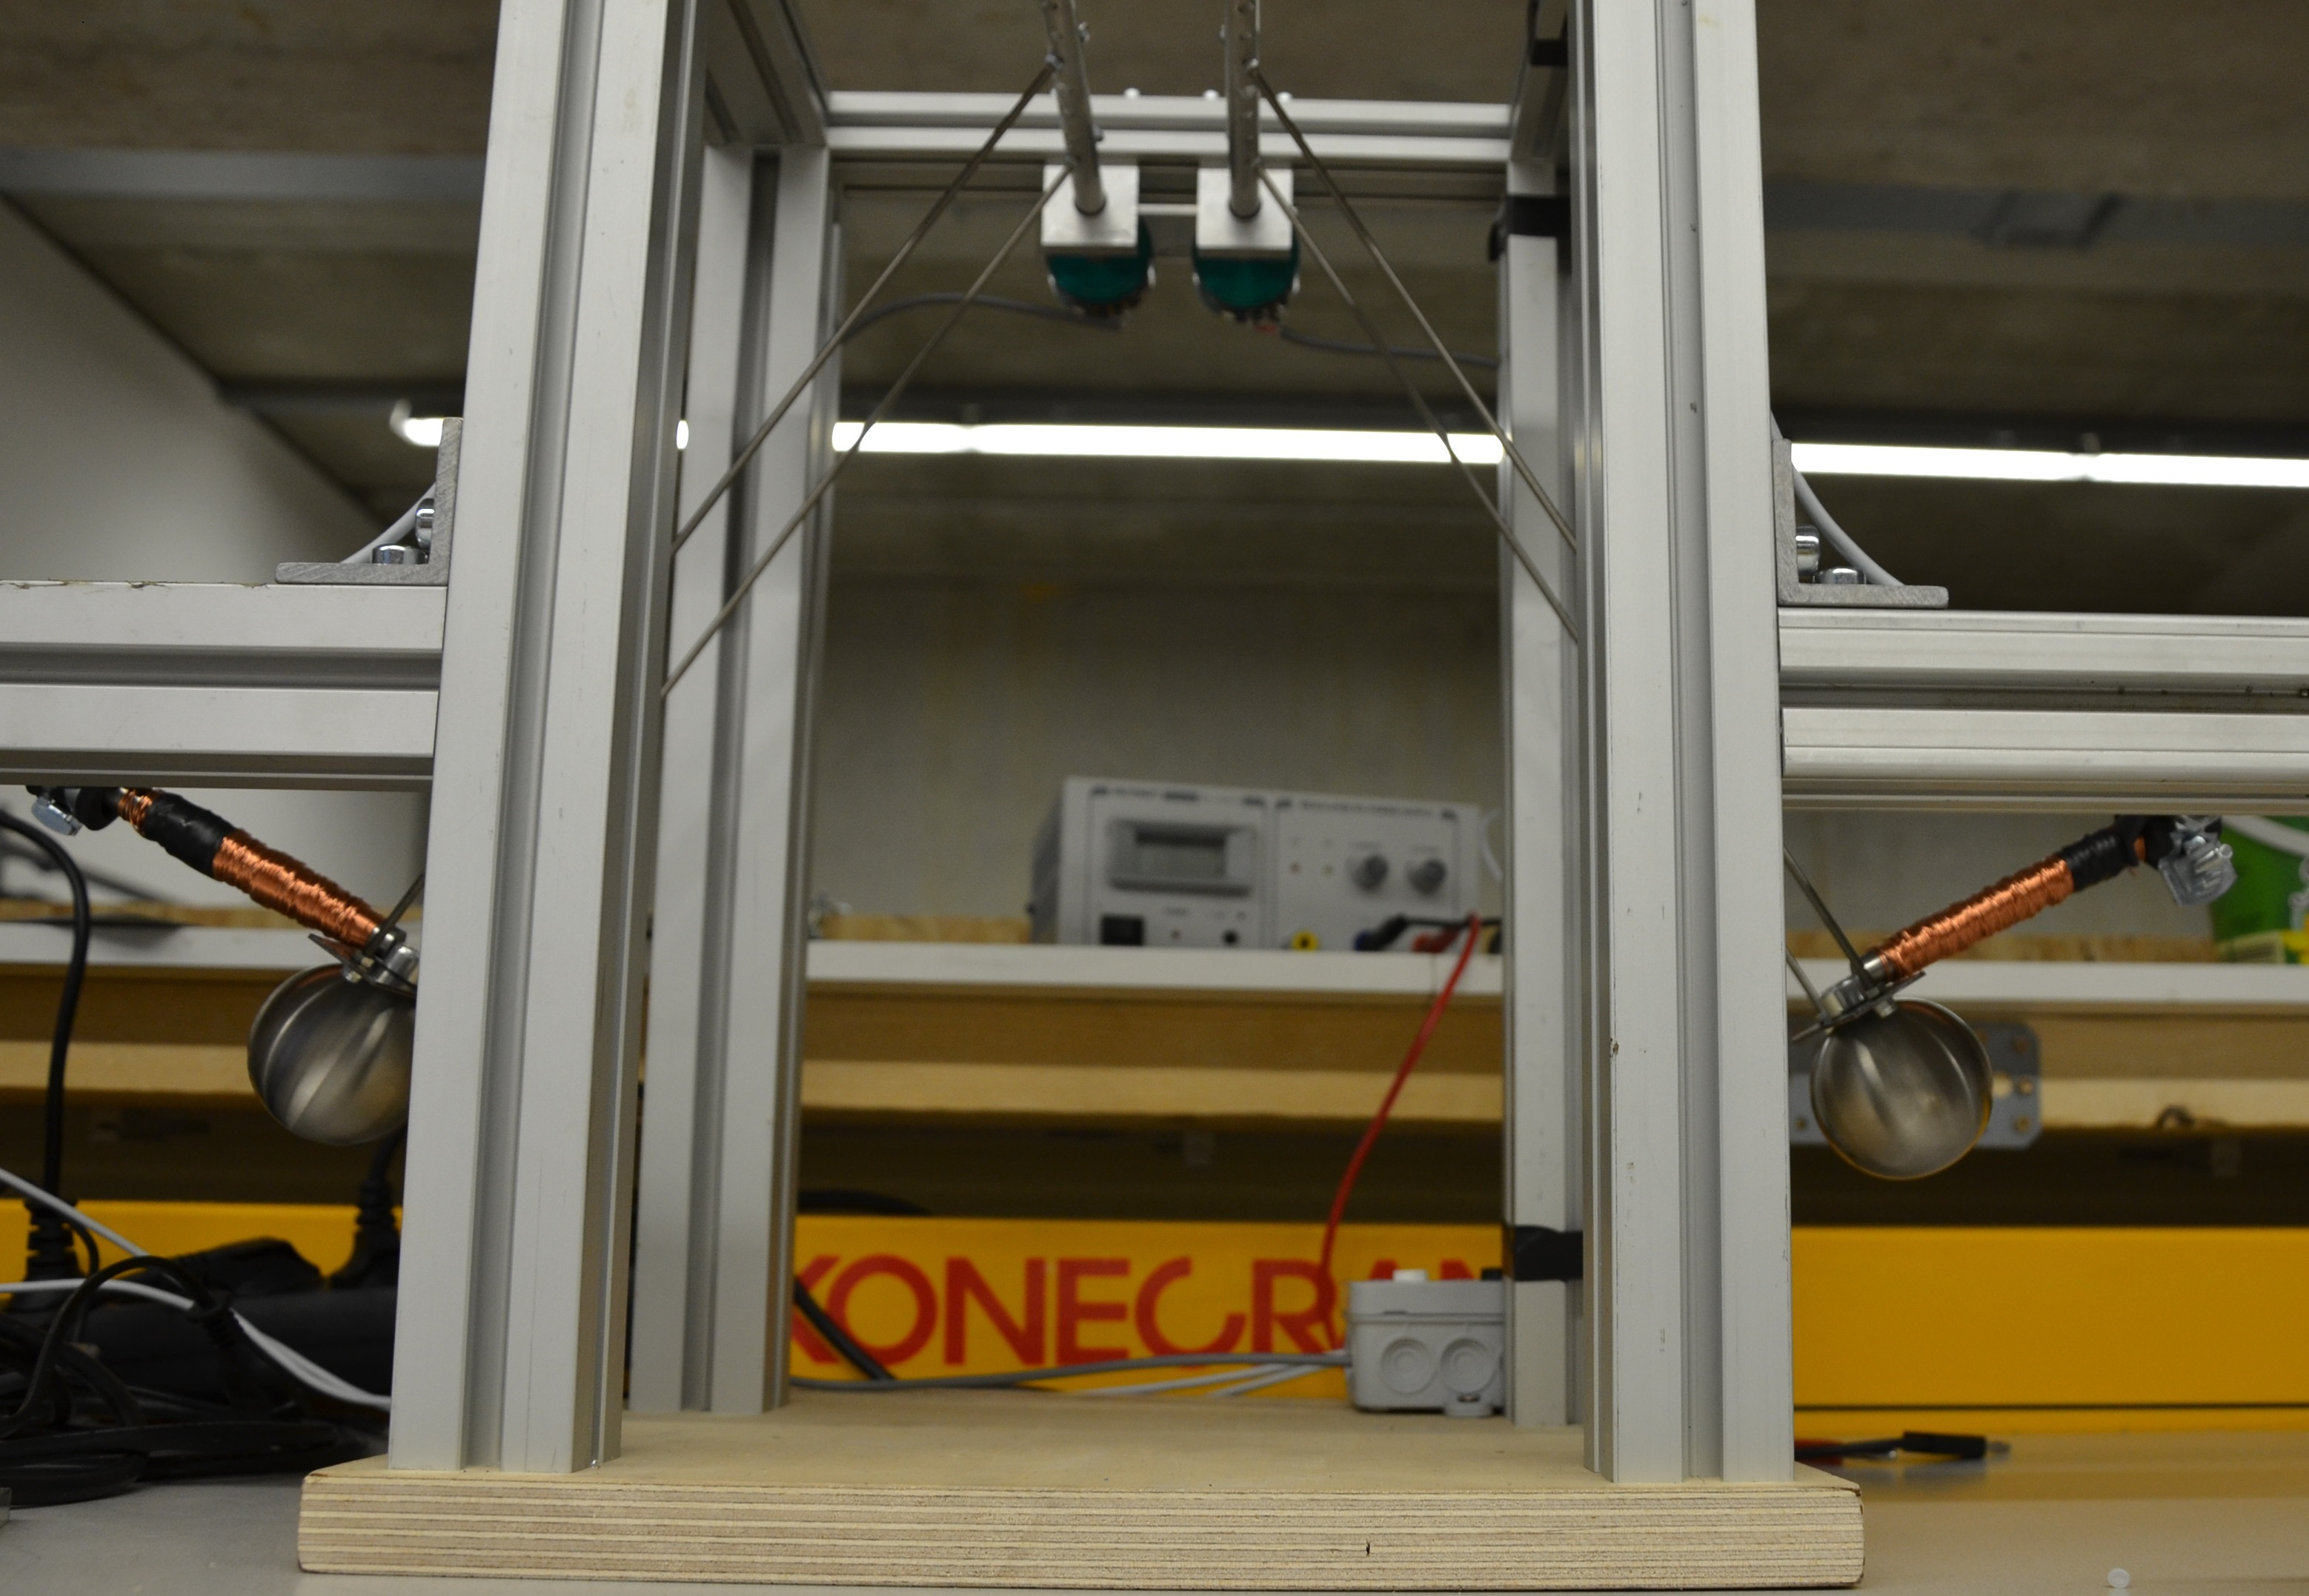
\includegraphics[width=.48\columnwidth]{007hollowspheredevice2}}  \quad
\subfloat[Coefficient of restitution of 2 mm silibeads]
{\label{fig:008esilibeads2mm2}%
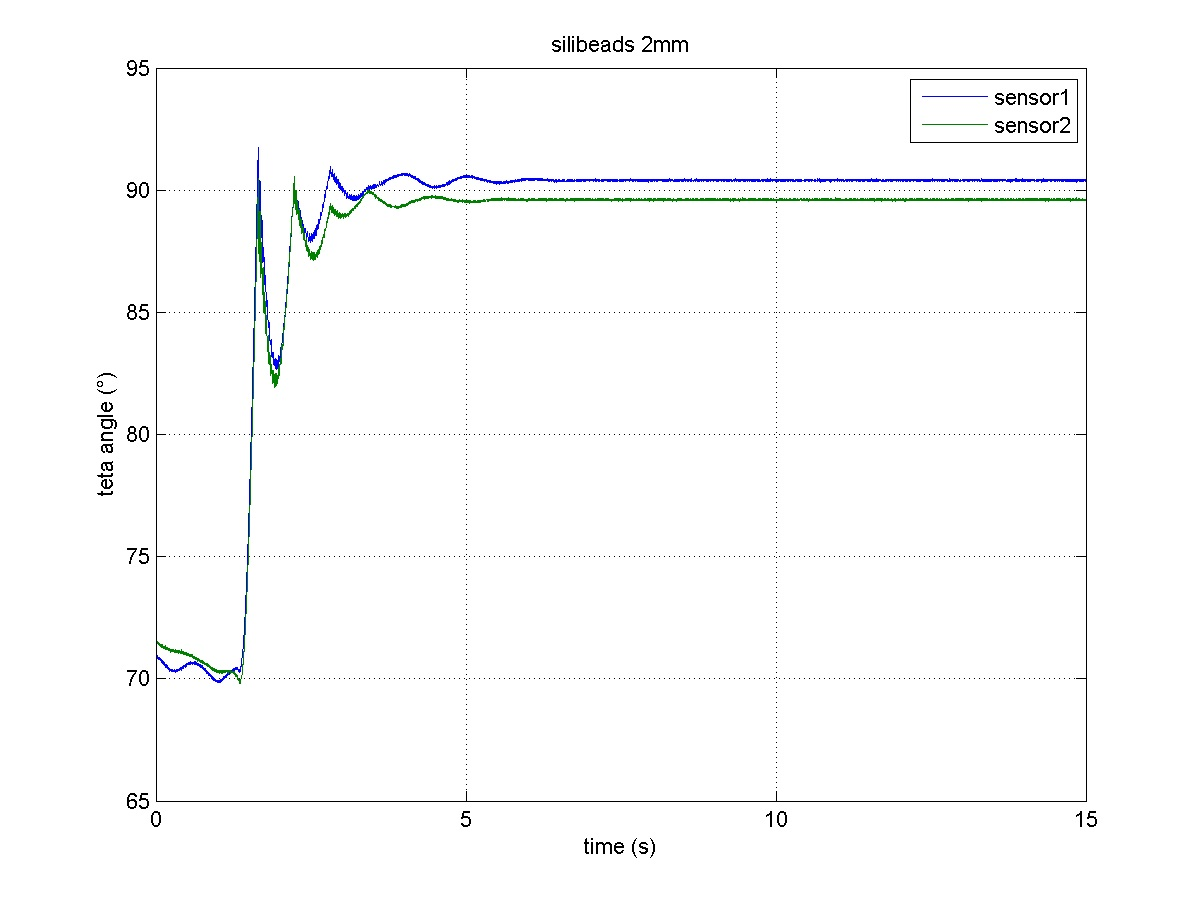
\includegraphics[width=.48\columnwidth]{008esilibeads2mm2}} \\
\caption[Hollow Spheres experiment]{Hollow Spheres experiment}
\label{fig:hollowspheres}
\end{figure}


Before start the spheres are kept at 40º from the vertical through magnetic rods, in order to avoid spin and torque when they are released.
After releasing the spheres move with a defined \ac{omega1}, calculated as the fraction of the angular displacement over time variation.
Then they collide and flee with an \ac{omega2}.\\

Now the results present little noise, as you can see in Figure \ref{fig:008esilibeads2mm2}.
Unfortunately the steel truss are transmitting vibration to the structure, I am trying to understand how much is the energy dissipation.\\

Soon I should receive a simulation script for this experiment.\\

%\subsubsection{HS}
%\label{subsubsection:hsexperiment}



%\subsubsection{HS simulation}
%\label{subsubsection:hssimulation}


%\input{Paragrafi/Newfloor}
%% !TEX encoding = UTF-8
% !TEX TS-program = pdflatex
% !TEX root = ../Articolo.tex
% !TEX spellcheck = it-IT

%************************************************
\section{Ipsum}
\label{sec:ipsum}
%************************************************


Lorem ipsum dolor sit amet, consectetuer adipiscing elit. Nam dui ligula, fringilla a, euismod sodales, sollicitudin vel, wisi. Morbi auctor lorem non justo. Nam lacus libero, pretium at, lobortis vitae, ultricies et, tellus.
\begin{description}
\item[Lorem ipsum dolor] sit amet, consectetuer adipiscing elit. Ut purus elit, vestibulum ut, placerat ac $\lim_{n \to \infty}\sum_{k=1}^n \frac{1}{k^2}= \frac{\pi^2}{6}$.
\item[Mauris ut leo.]
Cras viverra metus rhoncus sem. Nulla et lectus vestibulum urna fringilla ultrices. Phasellus eu tellus sit amet tortor gravida placerat.
\[
\lim_{n \to \infty}\sum_{k=1}^n \frac{1}{k^2}= \frac{\pi^2}{6}.
\]
\end{description}

Nulla malesuada porttitor diam. Donec felis erat, congue non, volutpat at, tincidunt tristique, libero. Vivamus viverra fermentum felis.
\begin{equation}
\label{eq:euler}
e^{i\pi}+1=0.
\end{equation}
Dalla formula~\eqref{eq:euler} 
si deduce che\dots






\subsection{Nozioni basilari}

\subsubsection{Insiemi numerici}

Donec nonummy pellentesque ante. Phasellus adipiscing semper elit.
\begin{equation}
x^2 \geq 0 \quad
\forall x \in \mathbb{R}.
\end{equation}


\subsubsection{Le matrici}

\lipsum[2]
\begin{equation}
A=
\begin{bmatrix}
x_{11} & x_{12} & \dots \\
x_{21} & x_{22} & \dots \\
\vdots & \vdots & \ddots
\end{bmatrix}
\end{equation}



\subsection{Formule fuori corpo}

Proin fermentum massa ac quam. Sed diam turpis, molestie vitae, placerat a, molestie nec, leo. Maecenas lacinia. Nam ipsum ligula, eleifend at, accumsan nec, suscipit a, ipsum. 


\subsubsection{Una formula spezzata con allineamento}

\lipsum[2]
\begin{equation} 
\begin{split} 
a &= b+c-d \\ 
  &= e-f \\ 
  &= g+h \\ 
  &= i. 
\end{split} 
\end{equation}

 
\subsubsection{Casi}

\lipsum[3]
\begin{equation}
f(n):=
\begin{cases} 
2n+1, & \text{con $n$ dispari,} \\ 
n/2,  & \text{con $n$ pari.} 
\end{cases} 
\end{equation}



\subsection{Enunciati e dimostrazioni}

Nunc eleifend consequat lorem. Sed lacinia nulla vitae enim. Pellentesque tincidunt purus vel magna. Integer non enim. Praesent euismod nunc eu purus.
\begin{definizione}[di Gauss] 
Un \emph{matematico} trova ovvio che
$\int_{-\infty}^{+\infty}
e^{-x^2}\,dx=\sqrt{\pi}$. 
\end{definizione} 
\begin{teorema} 
I matematici, se ce ne sono, sono molto rari.
\end{teorema} 

\lipsum[2]

\begin{teorema}[di Pitagora]
La somma dei quadrati costruiti sui cateti uguaglia il quadrato costruito sull'ipotenusa.
\end{teorema}
La dimostrazione viene lasciata per esercizio.

Donec bibendum quam in tellus. Nullam cursus pulvinar lectus. Donec et mi. Nam vulputate metus eu enim. Vestibulum pellentesque felis eu massa.
\begin{teorema}[Sorpresa]
Si ha che $\log(-1)^2=2\log(-1)$.
\end{teorema} 
\begin{proof} 
Si ha che $\log(1)^2 = 2\log(1)$.
Ma si ha anche che $\log(-1)^2=\log(1)=0$.
Quindi $2\log(-1)=0$, da cui la tesi.
\end{proof}
Viene un quadratino a fine dimostrazione.
\begin{legge}
\label{lex:capo}
Il capo ha ragione.
\end{legge}
\begin{decreto}[Aggiornamento alla legge~\ref{lex:capo}]
Il capo ha \emph{sempre} ragione.
\end{decreto}
\begin{legge}
Se il capo ha torto, vedere la 
legge~\ref{lex:capo}.
\end{legge}


Nam dui ligula, fringilla a, euismod sodales, sollicitudin vel, wisi. Morbi auctor lorem non justo. Nam lacus libero, pretium at, lobortis vitae, ultricies et, tellus.
\begin{murphy}
Cras nec ante. Pellentesque a nulla. Cum sociis natoque penatibus et magnis dis parturient montes, nascetur ridiculus mus. Aliquam tincidunt urna.
\end{murphy}

%\input{Paragrafi/trota}
\appendix
%% !TEX encoding = UTF-8
% !TEX TS-program = pdflatex
% !TEX root = ../Articolo.tex
% !TEX spellcheck = it-IT

%************************************************
\section{Dolor}
\label{sec:dolor}
%************************************************

\lipsum[1]

\subsection{Mane}
\lipsum[2]

\subsection{Tekel}
\lipsum[3]

\subsection{Fares}
\lipsum[4-5]

% *****************************************************************
% Materiale finale
%% !TEX encoding = UTF-8
% !TEX TS-program = pdflatex
% !TEX root = ../Articolo.tex
% !TEX spellcheck = it-IT

%************************************************
\section{Acronyms list}
\label{sec:acro}
%************************************************
%*******************************************************
% Elenco degli acronimi
%*******************************************************

		
\begin{acronym}[TDMA]
%\acro{CDMA}{Code Division Multiple Access}
%\acro{GSM}{Global System for Mobile communication}
%\acro{NA}[\ensuremath{N_{\mathrm A}}]{Number of Avogadro\acroextra{ (see \S\ref{Chem})}}
%\acro{NAD+}[NAD\textsuperscript{+}]{Nicotinamide Adenine Dinucleotide}
%\acro{NUA}{Not Used Acronym}
%\acro{TDMA}{Time Division Multiple Access}
%\acro{UA}{Used Acronym}
%\acro{lox}[\ensuremath{LOX}]{Liquid Oxygen}%
%\acro{lh2}[\ensuremath{LH_2}]{Liquid Hydrogen}%
%\acro{IC}{Integrated Circuit}%
%\acro{BUT}{Block Under Test}%
%\acrodefplural{BUT}{Blocks Under Test}%

\acro{phis}[$\phi_s$]{angle of sliding friction}
\acro{aor}[$AOR$]{Angle of repose}
\acro{omega1}[$\omega_1$]{angular speed before first impact}
\acro{omega2}[$\omega_2$]{angular speed after first impact}
\acro{omega3}[$\omega_3$]{angular speed before second impact}
\acro{omega4}[$\omega_4$]{angular speed after second impact}
\acro{dem}[$DEM$]{Discrete Element Method}
\acro{euno}[$e_1$]{coefficient of first restitution}
\acro{cor}[$COR$]{coefficient of restitution}
\acro{edue}[$e_2$]{coefficient of second restitution}
\acro{mu}[$\mu_s$]{coefficient of sliding friction}
\acro{mur}[$\mu_r$]{coefficient of static rolling friction}
\acro{jsct}[$JSCT$]{Jenike Shear Cell tester}
\acro{pmsct}[$PMSCT$]{``Poor Man'' Shear Cell tester}
\acro{liggghts}[$LIGGGHTS$]{LAMMPS improved for general granular and granular heat transfer simulations}
\acro{r}[$r$]{radius of the particle}
\acro{ra}[$R$]{external radius of the sphere}
\acro{sasct}[$SASCT$]{Schulze Annular Shear Cell tester}

\end{acronym}

%% !TEX encoding = UTF-8
% !TEX TS-program = pdflatex
% !TEX root = ../Articolo.tex
% !TEX spellcheck = it-IT

%*******************************************************
% Bibliografia
%*******************************************************
%\nocite{*}
\printbibliography
%******************************************************************
\end{document}


